\documentclass[12pt,a4paper,oneside]{report}
\usepackage[utf8]{inputenc}
\usepackage[T1]{fontenc}
\usepackage[english]{babel}
\usepackage{lmodern,microtype,setspace,geometry}
\geometry{margin=2.5cm}
\onehalfspacing
\usepackage{graphicx,xcolor,booktabs,longtable,array,enumitem,float}
\usepackage{listings,caption,subcaption}
\usepackage{tikz}
\usetikzlibrary{arrows.meta,positioning,shapes.geometric,fit,matrix,backgrounds,calc}
\usepackage{hyperref}
\def\UrlBreaks{\do\/\do\-\do\_\do\{\do\}}
\hypersetup{colorlinks=true,linkcolor=blue!55!black,citecolor=blue!55!black,
urlcolor=blue!65!black,pdftitle={EduFlex Mobile Learning Platform}}

\definecolor{eduflexteal}{HTML}{00796B}
\definecolor{codegray}{HTML}{F4F6F8}
\lstset{backgroundcolor=\color{codegray},basicstyle=\ttfamily\small,
breaklines=true,frame=single,showstringspaces=false,numbers=left,
numberstyle=\tiny\color{black!45},numbersep=8pt}

% Replace these values before submission.
\newcommand{\projectname}{EduFlex}
\newcommand{\university}{University of Science}
\newcommand{\faculty}{Faculty of Information Technology}
\newcommand{\studentname}{Vu Thanh Dat}
\newcommand{\studentid}{23127346}
\newcommand{\supervisor}{Dr.\ Truong Toan Thinh}
\newcommand{\submissiondate}{[Month Year]}

% Diagram commands used by main.tex. All figures are native TikZ so the
% Overleaf package does not depend on generated image files.

\newcommand{\systemcontextdiagram}{
\begin{figure}[H]\centering
\resizebox{0.94\textwidth}{!}{
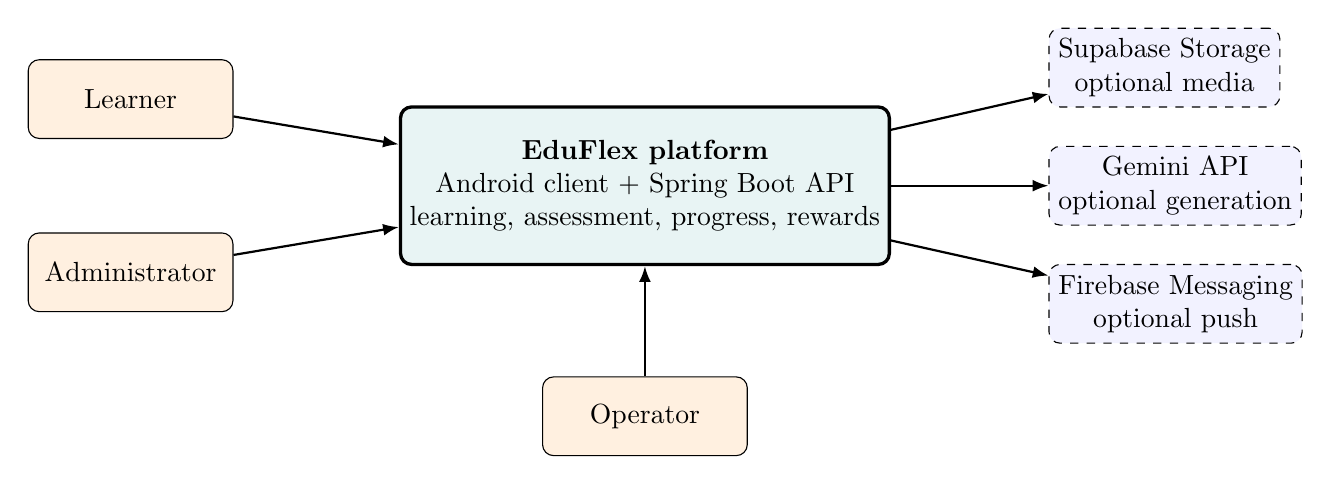
\begin{tikzpicture}[
person/.style={draw,rounded corners,fill=orange!12,align=center,minimum width=2.6cm,minimum height=1cm},
system/.style={draw,rounded corners,very thick,fill=teal!9,align=center,minimum width=4.5cm,minimum height=2cm},
external/.style={draw,dashed,rounded corners,fill=blue!5,align=center,minimum width=2.8cm,minimum height=1cm},
arr/.style={-{Latex[length=2mm]},thick}]
\node[system](platform){\textbf{EduFlex platform}\\Android client + Spring Boot API\\learning, assessment, progress, rewards};
\node[person,left=2.1cm of platform,yshift=1.1cm](learner){Learner};
\node[person,left=2.1cm of platform,yshift=-1.1cm](admin){Administrator};
\node[person,below=1.4cm of platform](operator){Operator};
\node[external,right=2cm of platform,yshift=1.5cm](supabase){Supabase Storage\\optional media};
\node[external,right=2cm of platform](gemini){Gemini API\\optional generation};
\node[external,right=2cm of platform,yshift=-1.5cm](firebase){Firebase Messaging\\optional push};
\draw[arr](learner)--(platform);
\draw[arr](admin)--(platform);
\draw[arr](operator)--(platform);
\draw[arr](platform)--(supabase);
\draw[arr](platform)--(gemini);
\draw[arr](platform)--(firebase);
\end{tikzpicture}}
\caption{System context and external actors}\label{fig:system-context}
\end{figure}}

\newcommand{\backendlayersdiagram}{
\begin{figure}[H]\centering
\resizebox{0.92\textwidth}{!}{
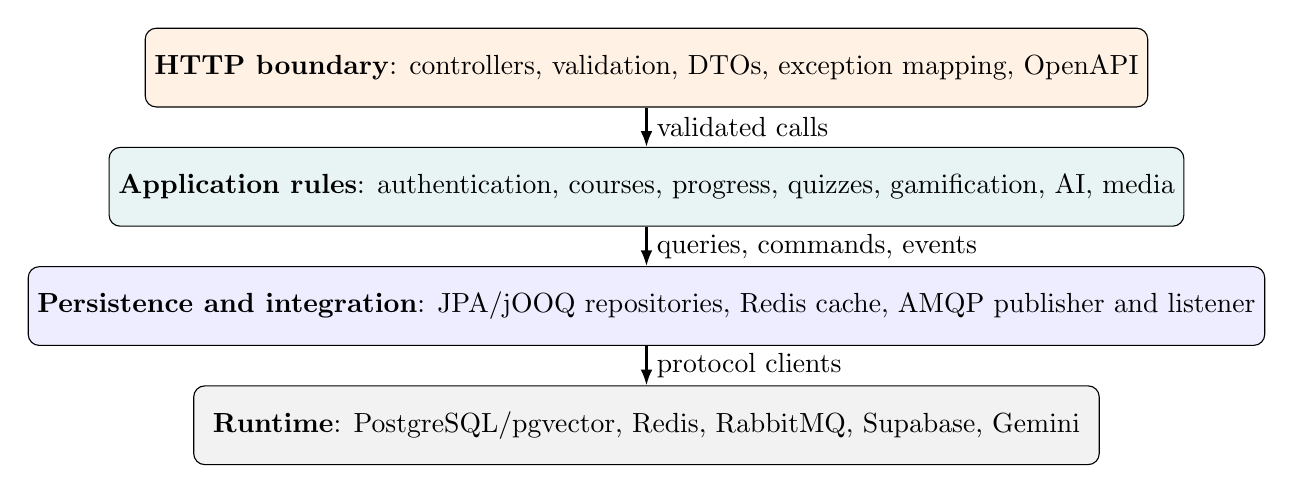
\begin{tikzpicture}[
layer/.style={draw,rounded corners,align=center,minimum width=11.5cm,minimum height=1cm},
arr/.style={-{Latex[length=2mm]},thick}]
\node[layer,fill=orange!10](http){\textbf{HTTP boundary}: controllers, validation, DTOs, exception mapping, OpenAPI};
\node[layer,fill=teal!9,below=.5cm of http](services){\textbf{Application rules}: authentication, courses, progress, quizzes, gamification, AI, media};
\node[layer,fill=blue!7,below=.5cm of services](repositories){\textbf{Persistence and integration}: JPA/jOOQ repositories, Redis cache, AMQP publisher and listener};
\node[layer,fill=gray!10,below=.5cm of repositories](runtime){\textbf{Runtime}: PostgreSQL/pgvector, Redis, RabbitMQ, Supabase, Gemini};
\draw[arr](http)--node[right]{validated calls}(services);
\draw[arr](services)--node[right]{queries, commands, events}(repositories);
\draw[arr](repositories)--node[right]{protocol clients}(runtime);
\end{tikzpicture}}
\caption{Backend responsibility layers}\label{fig:backend-layers}
\end{figure}}

\newcommand{\androidnavigationdiagram}{
\begin{figure}[H]\centering
\resizebox{\textwidth}{!}{
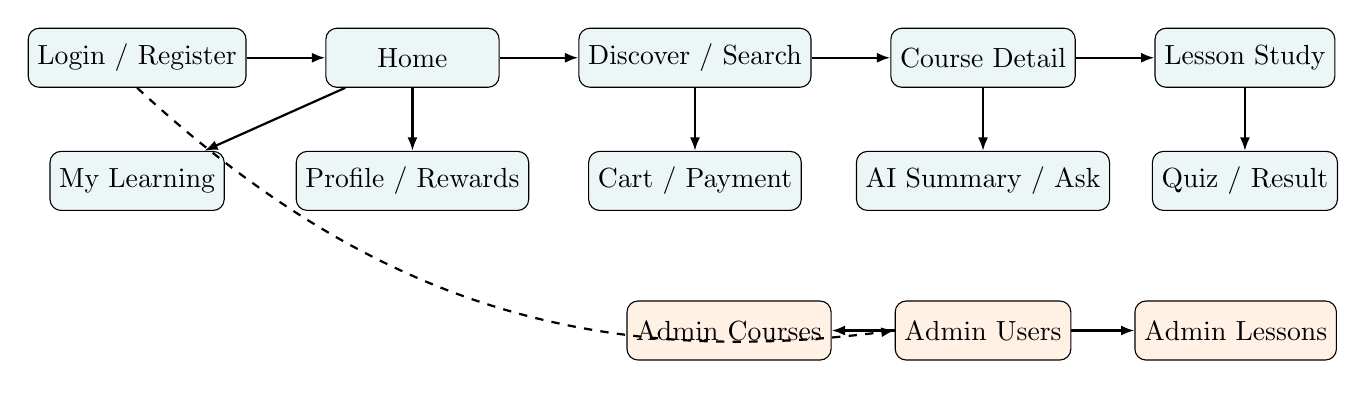
\begin{tikzpicture}[
screen/.style={draw,rounded corners,fill=teal!7,align=center,minimum width=2.2cm,minimum height=.75cm},
admin/.style={draw,rounded corners,fill=orange!10,align=center,minimum width=2.2cm,minimum height=.75cm},
arr/.style={-{Latex[length=1.7mm]},thick}]
\node[screen](auth){Login / Register};
\node[screen,right=1cm of auth](home){Home};
\node[screen,right=1cm of home](discover){Discover / Search};
\node[screen,right=1cm of discover](detail){Course Detail};
\node[screen,right=1cm of detail](lesson){Lesson Study};
\node[screen,below=.8cm of lesson](quiz){Quiz / Result};
\node[screen,below=.8cm of detail](ai){AI Summary / Ask};
\node[screen,below=.8cm of discover](cart){Cart / Payment};
\node[screen,below=.8cm of home](profile){Profile / Rewards};
\node[screen,below=.8cm of auth](learn){My Learning};
\node[admin,below=2.7cm of detail](adminhome){Admin Users};
\node[admin,left=.8cm of adminhome](admincourses){Admin Courses};
\node[admin,right=.8cm of adminhome](adminlessons){Admin Lessons};
\draw[arr](auth)--(home);\draw[arr](home)--(discover);\draw[arr](discover)--(detail);
\draw[arr](detail)--(lesson);\draw[arr](lesson)--(quiz);\draw[arr](detail)--(ai);
\draw[arr](discover)--(cart);\draw[arr](home)--(profile);\draw[arr](home)--(learn);
\draw[arr,dashed](auth.south)to[bend right=25](adminhome.west);
\draw[arr](adminhome)--(admincourses);\draw[arr](adminhome)--(adminlessons);
\end{tikzpicture}}
\caption{Android navigation and principal user journeys}\label{fig:android-navigation}
\end{figure}}

\newcommand{\deploymentdiagram}{
\begin{figure}[H]\centering
\resizebox{\textwidth}{!}{
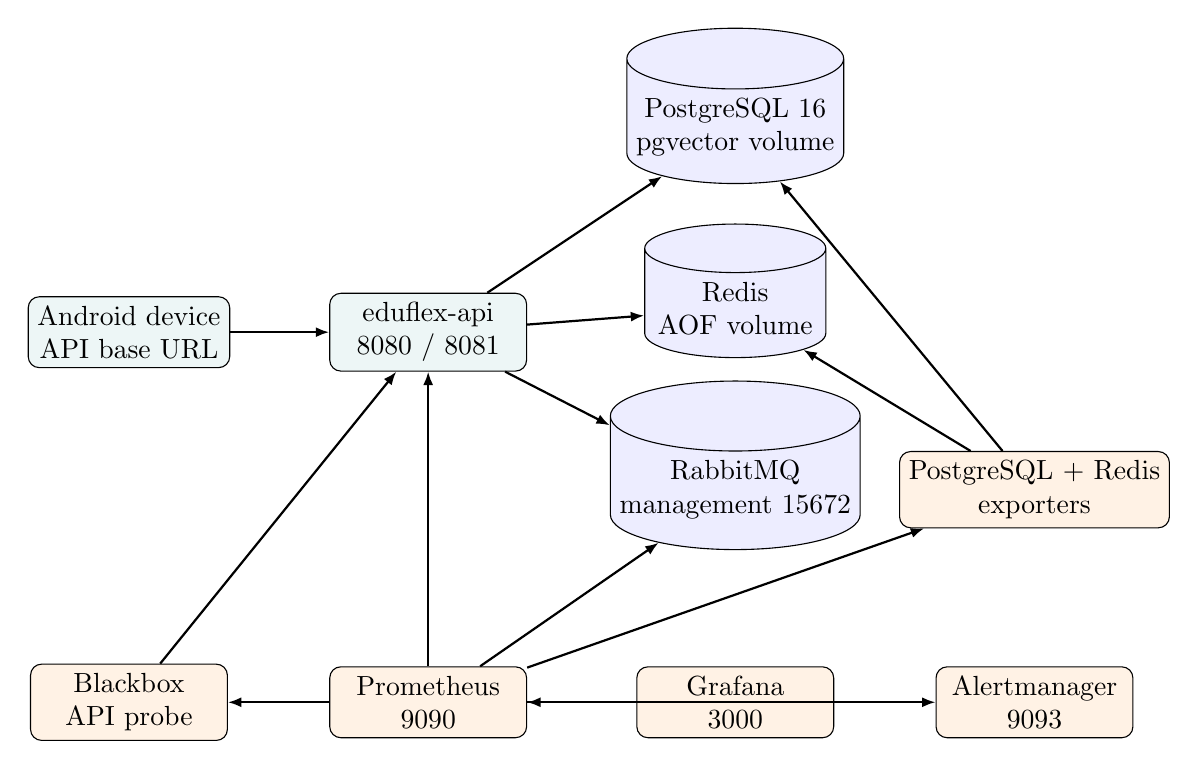
\begin{tikzpicture}[
svc/.style={draw,rounded corners,align=center,minimum width=2.5cm,minimum height=.9cm,fill=teal!7},
obs/.style={draw,rounded corners,align=center,minimum width=2.5cm,minimum height=.9cm,fill=orange!10},
store/.style={draw,cylinder,shape border rotate=90,aspect=.28,align=center,minimum width=2.3cm,minimum height=1cm,fill=blue!7},
arr/.style={-{Latex[length=1.7mm]},thick}]
\node[svc] at (0,2.4)(android){Android device\\API base URL};
\node[svc] at (3.8,2.4)(api){eduflex-api\\8080 / 8081};
\node[store] at (7.7,5.0)(pg){PostgreSQL 16\\pgvector volume};
\node[store] at (7.7,2.7)(redis){Redis\\AOF volume};
\node[store] at (7.7,.4)(rabbit){RabbitMQ\\management 15672};
\node[obs] at (0,-2.3)(blackbox){Blackbox\\API probe};
\node[obs] at (3.8,-2.3)(prom){Prometheus\\9090};
\node[obs] at (7.7,-2.3)(grafana){Grafana\\3000};
\node[obs] at (11.5,-2.3)(alert){Alertmanager\\9093};
\node[obs] at (11.5,.4)(exporters){PostgreSQL + Redis\\exporters};
\draw[arr](android)--(api);\draw[arr](api)--(pg);\draw[arr](api)--(redis);\draw[arr](api)--(rabbit);
\draw[arr](prom)--(blackbox);\draw[arr](blackbox)--(api);
\draw[arr](prom)--(api);\draw[arr](prom)--(exporters);
\draw[arr](exporters)--(pg);\draw[arr](exporters)--(redis);
\draw[arr](prom)--(rabbit);\draw[arr](grafana)--(prom);
\draw[arr](prom)--(alert);
\end{tikzpicture}}
\caption{Docker Compose deployment and monitoring topology}\label{fig:deployment}
\end{figure}}

\newcommand{\erdmodeldiagram}{
\begin{figure}[H]\centering
\resizebox{\textwidth}{!}{
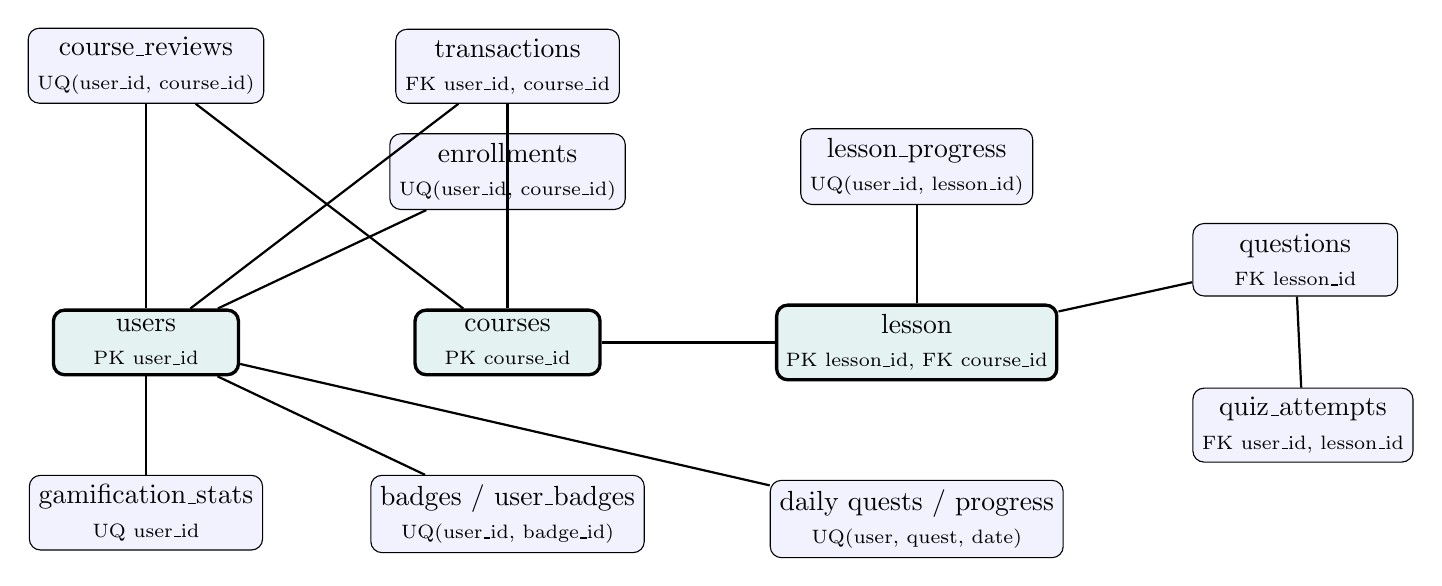
\begin{tikzpicture}[
entity/.style={draw,rounded corners,fill=blue!5,align=center,minimum width=2.6cm,minimum height=.92cm},
core/.style={draw,rounded corners,fill=teal!10,very thick,align=center,minimum width=2.35cm,minimum height=.82cm},
rel/.style={thick}]
\node[core](users){users\\\scriptsize PK user\_id};
\node[core,right=2.2cm of users](courses){courses\\\scriptsize PK course\_id};
\node[core,right=2.2cm of courses](lessons){lesson\\\scriptsize PK lesson\_id, FK course\_id};
\node[entity,above=1.25cm of courses](enrol){enrollments\\\scriptsize UQ(user\_id, course\_id)};
\node[entity,above=1.25cm of lessons](progress){lesson\_progress\\\scriptsize UQ(user\_id, lesson\_id)};
\node[entity,right=1.7cm of lessons,yshift=1.05cm](questions){questions\\\scriptsize FK lesson\_id};
\node[entity,right=1.7cm of lessons,yshift=-1.05cm](attempts){quiz\_attempts\\\scriptsize FK user\_id, lesson\_id};
\node[entity,below=1.25cm of users](stats){gamification\_stats\\\scriptsize UQ user\_id};
\node[entity,below=1.25cm of courses](badges){badges / user\_badges\\\scriptsize UQ(user\_id, badge\_id)};
\node[entity,below=1.25cm of lessons](quests){daily quests / progress\\\scriptsize UQ(user, quest, date)};
\node[entity,above=2.6cm of users](reviews){course\_reviews\\\scriptsize UQ(user\_id, course\_id)};
\node[entity,above=2.6cm of courses](payments){transactions\\\scriptsize FK user\_id, course\_id};
\draw[rel](users)--(enrol);\draw[rel](courses)--(enrol);
\draw[rel](courses)--(lessons);\draw[rel](lessons)--(progress);
\draw[rel](lessons)--(questions);\draw[rel](questions)--(attempts);
\draw[rel](users)--(stats);\draw[rel](users)--(badges);\draw[rel](users)--(quests);
\draw[rel](users)--(reviews);\draw[rel](courses)--(reviews);
\draw[rel](users)--(payments);\draw[rel](courses)--(payments);
\end{tikzpicture}}
\caption{Logical database relationship model}\label{fig:erd}
\end{figure}}

\newcommand{\apiboundarydiagram}{
\begin{figure}[H]\centering
\resizebox{\textwidth}{!}{
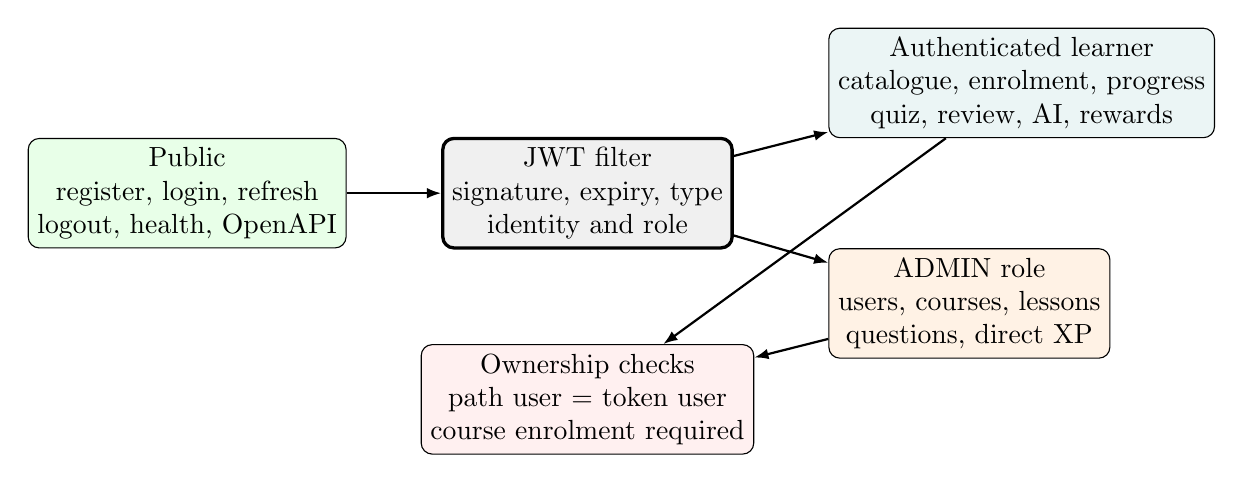
\begin{tikzpicture}[
group/.style={draw,rounded corners,align=center,minimum width=3.4cm,minimum height=1.05cm},
gate/.style={draw,very thick,rounded corners,fill=gray!12,align=center,minimum width=3.5cm,minimum height=1.1cm},
arr/.style={-{Latex[length=1.8mm]},thick}]
\node[group,fill=green!9](public){Public\\register, login, refresh\\logout, health, OpenAPI};
\node[gate,right=1.2cm of public](filter){JWT filter\\signature, expiry, type\\identity and role};
\node[group,fill=teal!8,right=1.2cm of filter,yshift=1.4cm](learner){Authenticated learner\\catalogue, enrolment, progress\\quiz, review, AI, rewards};
\node[group,fill=orange!10,right=1.2cm of filter,yshift=-1.4cm](admin){ADMIN role\\users, courses, lessons\\questions, direct XP};
\node[group,fill=red!6,below=1.2cm of filter](ownership){Ownership checks\\path user = token user\\course enrolment required};
\draw[arr](public)--(filter);
\draw[arr](filter)--(learner);
\draw[arr](filter)--(admin);
\draw[arr](learner)--(ownership);\draw[arr](admin)--(ownership);
\end{tikzpicture}}
\caption{API groups and authorization boundaries}\label{fig:api-boundaries}
\end{figure}}

\newcommand{\authsequencediagram}{
\begin{figure}[H]\centering
\resizebox{0.96\textwidth}{!}{
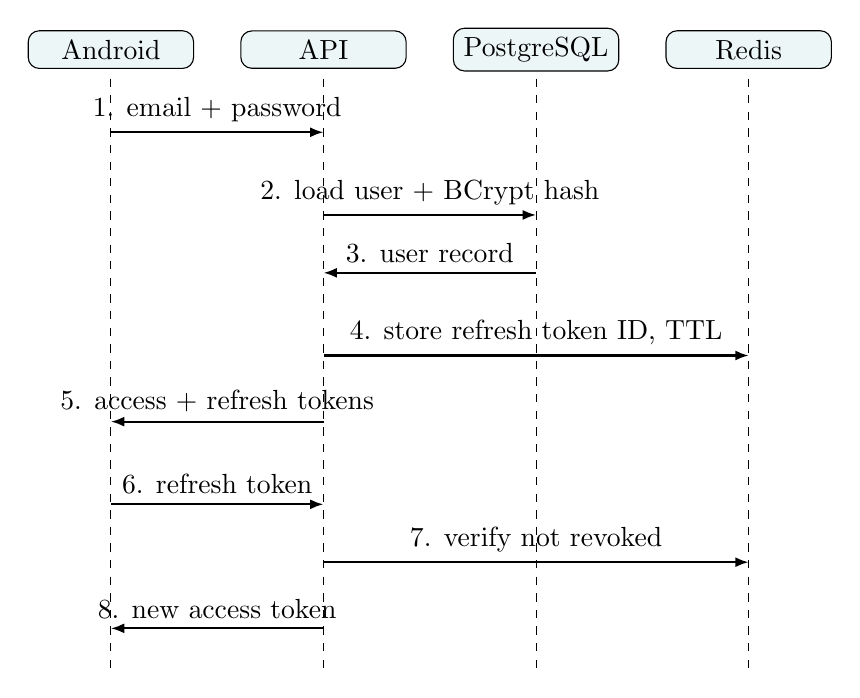
\begin{tikzpicture}[x=2.7cm,y=1.05cm,arr/.style={-{Latex[length=1.7mm]},thick}]
\foreach \x/\name in {0/Android,1/API,2/PostgreSQL,3/Redis}
  {\node[draw,rounded corners,fill=teal!7,minimum width=2.1cm] at (\x,0) {\name};
   \draw[dashed] (\x,-.35)--(\x,-7.5);}
\draw[arr](0,-1)--node[above]{1. email + password}(1,-1);
\draw[arr](1,-2)--node[above]{2. load user + BCrypt hash}(2,-2);
\draw[arr](2,-2.7)--node[above]{3. user record}(1,-2.7);
\draw[arr](1,-3.7)--node[above]{4. store refresh token ID, TTL}(3,-3.7);
\draw[arr](1,-4.5)--node[above]{5. access + refresh tokens}(0,-4.5);
\draw[arr](0,-5.5)--node[above]{6. refresh token}(1,-5.5);
\draw[arr](1,-6.2)--node[above]{7. verify not revoked}(3,-6.2);
\draw[arr](1,-7)--node[above]{8. new access token}(0,-7);
\end{tikzpicture}}
\caption{Login and access-token refresh sequence}\label{fig:auth-sequence}
\end{figure}}

\newcommand{\learnerjourneydiagram}{
\begin{figure}[H]\centering
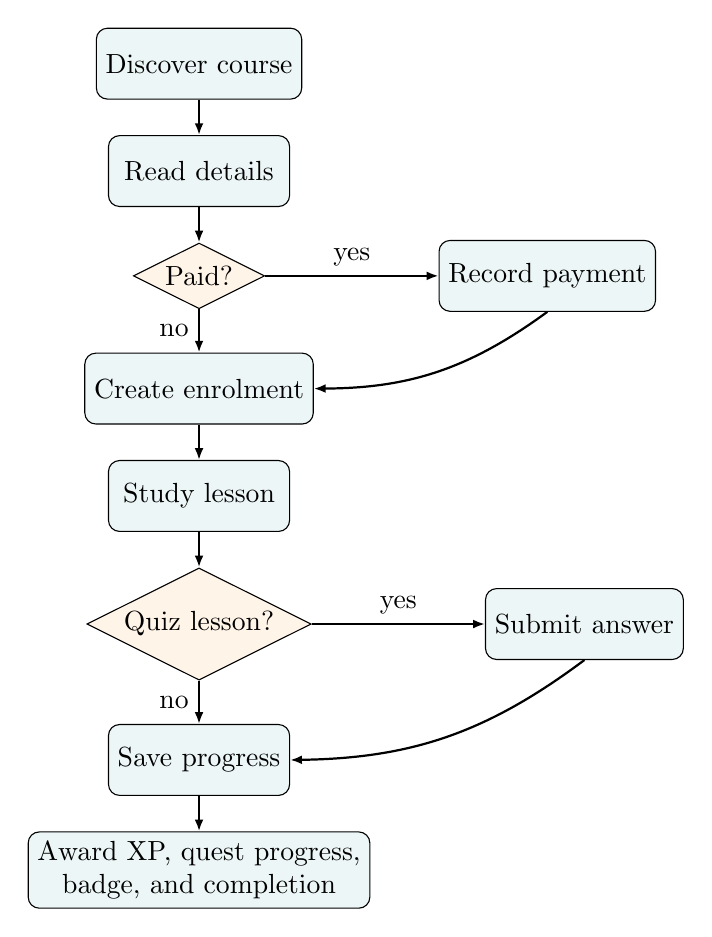
\begin{tikzpicture}[
state/.style={draw,rounded corners,fill=teal!7,align=center,minimum width=2.3cm,minimum height=.9cm},
decision/.style={draw,diamond,aspect=2,fill=orange!9,align=center,inner sep=1.5pt},
arr/.style={-{Latex[length=1.5mm]},thick}]
\node[state](discover){Discover course};
\node[state,below=.45cm of discover](detail){Read details};
\node[decision,below=.45cm of detail](paid){Paid?};
\node[state,right=2.2cm of paid](payment){Record payment};
\node[state,below=.55cm of paid](enrol){Create enrolment};
\node[state,below=.45cm of enrol](study){Study lesson};
\node[decision,below=.45cm of study](quiz){Quiz lesson?};
\node[state,right=2.2cm of quiz](submit){Submit answer};
\node[state,below=.55cm of quiz](complete){Save progress};
\node[state,below=.45cm of complete](reward){Award XP, quest progress,\\badge, and completion};
\draw[arr](discover)--(detail);\draw[arr](detail)--(paid);
\draw[arr](paid)--node[above]{yes}(payment);\draw[arr](payment.south)to[bend left=18](enrol.east);
\draw[arr](paid)--node[left]{no}(enrol);\draw[arr](enrol)--(study);
\draw[arr](study)--(quiz);\draw[arr](quiz)--node[above]{yes}(submit);
\draw[arr](submit.south)to[bend left=18](complete.east);\draw[arr](quiz)--node[left]{no}(complete);
\draw[arr](complete)--(reward);
\end{tikzpicture}
\caption{End-to-end learner course journey}\label{fig:learner-journey}
\end{figure}}

\newcommand{\progressstatediagram}{
\begin{figure}[H]\centering
\resizebox{0.9\textwidth}{!}{
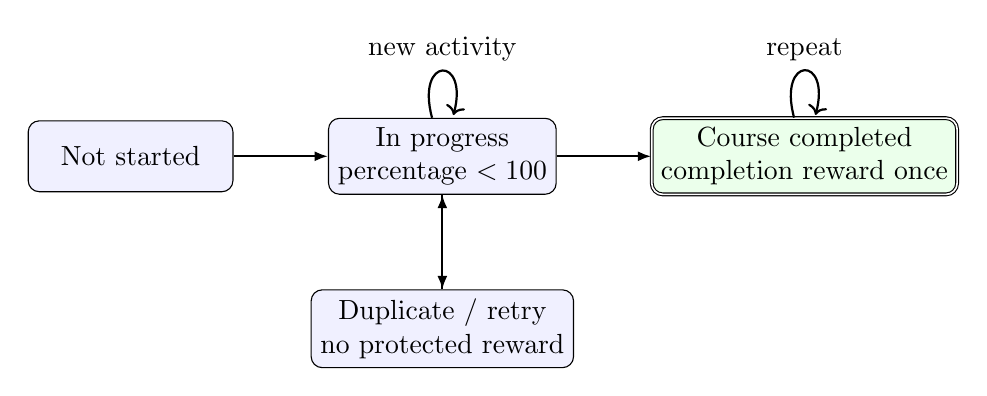
\begin{tikzpicture}[
state/.style={draw,rounded corners,fill=blue!6,align=center,minimum width=2.6cm,minimum height=.9cm},
terminal/.style={draw,double,rounded corners,fill=green!8,align=center,minimum width=2.6cm,minimum height=.9cm},
arr/.style={-{Latex[length=1.7mm]},thick}]
\node[state](notstarted){Not started};
\node[state,right=1.2cm of notstarted](inprogress){In progress\\percentage $<100$};
\node[terminal,right=1.2cm of inprogress](complete){Course completed\\completion reward once};
\node[state,below=1.2cm of inprogress](retry){Duplicate / retry\\no protected reward};
\draw[arr](notstarted)--(inprogress);
\draw[arr](inprogress)edge[loop above]node{new activity}(inprogress);
\draw[arr](inprogress)--(complete);
\draw[arr](complete)edge[loop above]node{repeat}(complete);
\draw[arr](inprogress)--(retry);
\draw[arr](retry)--(inprogress);
\end{tikzpicture}}
\caption{Learning-progress state and retry behavior}\label{fig:progress-state}
\end{figure}}

\newcommand{\cacheflowdiagram}{
\begin{figure}[H]\centering
\resizebox{0.94\textwidth}{!}{
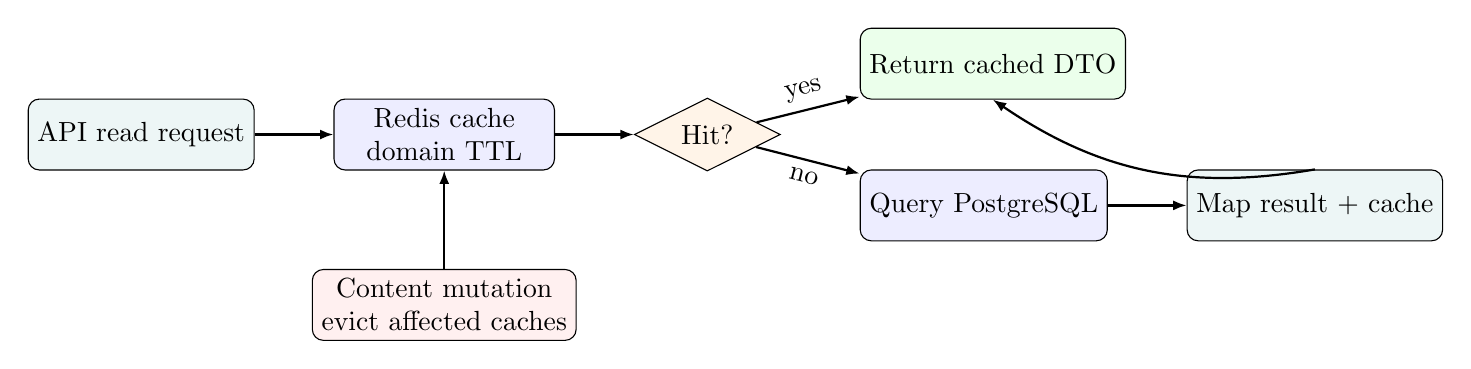
\begin{tikzpicture}[
box/.style={draw,rounded corners,align=center,minimum width=2.8cm,minimum height=.9cm},
decision/.style={draw,diamond,aspect=2,fill=orange!9,align=center},
arr/.style={-{Latex[length=1.7mm]},thick}]
\node[box,fill=teal!7](request){API read request};
\node[box,fill=blue!7,right=1cm of request](redis){Redis cache\\domain TTL};
\node[decision,right=1cm of redis](hit){Hit?};
\node[box,fill=green!8,right=1cm of hit,yshift=.9cm](return){Return cached DTO};
\node[box,fill=blue!7,right=1cm of hit,yshift=-.9cm](db){Query PostgreSQL};
\node[box,fill=teal!7,right=1cm of db](populate){Map result + cache};
\node[box,fill=red!6,below=1.25cm of redis](mutation){Content mutation\\evict affected caches};
\draw[arr](request)--(redis);\draw[arr](redis)--(hit);
\draw[arr](hit)--node[above,sloped]{yes}(return);
\draw[arr](hit)--node[below,sloped]{no}(db);\draw[arr](db)--(populate);
\draw[arr,bend left=22](populate.north)to(return.south);
\draw[arr](mutation)--(redis);
\end{tikzpicture}}
\caption{Cache-aside read and invalidation flow}\label{fig:cache-flow}
\end{figure}}

\newcommand{\embeddingsequencediagram}{
\begin{figure}[H]\centering
\resizebox{\textwidth}{!}{
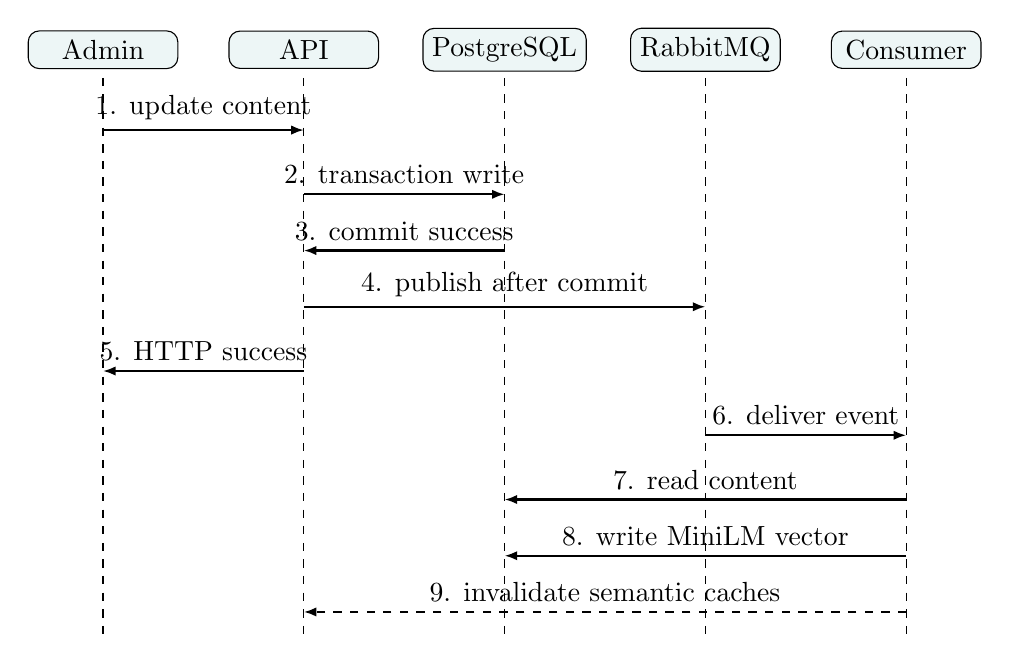
\begin{tikzpicture}[x=2.55cm,y=1.02cm,arr/.style={-{Latex[length=1.6mm]},thick}]
\foreach \x/\name in {0/Admin,1/API,2/PostgreSQL,3/RabbitMQ,4/Consumer}
  {\node[draw,rounded corners,fill=teal!7,minimum width=1.9cm] at (\x,0) {\name};
   \draw[dashed] (\x,-.35)--(\x,-7.3);}
\draw[arr](0,-1)--node[above]{1. update content}(1,-1);
\draw[arr](1,-1.8)--node[above]{2. transaction write}(2,-1.8);
\draw[arr](2,-2.5)--node[above]{3. commit success}(1,-2.5);
\draw[arr](1,-3.2)--node[above]{4. publish after commit}(3,-3.2);
\draw[arr](1,-4)--node[above]{5. HTTP success}(0,-4);
\draw[arr](3,-4.8)--node[above]{6. deliver event}(4,-4.8);
\draw[arr](4,-5.6)--node[above]{7. read content}(2,-5.6);
\draw[arr](4,-6.3)--node[above]{8. write MiniLM vector}(2,-6.3);
\draw[arr,dashed](4,-7)--node[above]{9. invalidate semantic caches}(1,-7);
\end{tikzpicture}}
\caption{Post-commit content embedding sequence}\label{fig:embedding-sequence}
\end{figure}}

\newcommand{\monitoringflowdiagram}{
\begin{figure}[H]\centering
\resizebox{0.96\textwidth}{!}{
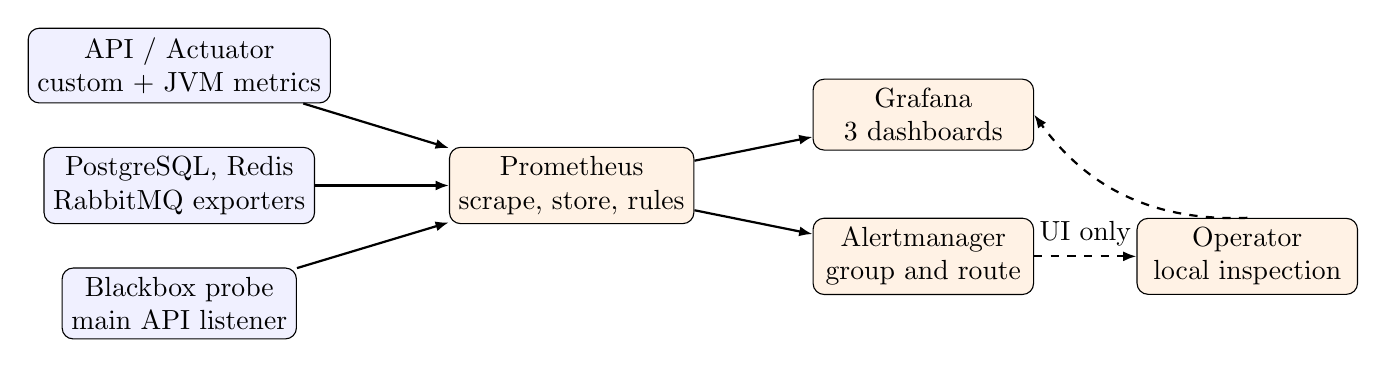
\begin{tikzpicture}[
source/.style={draw,rounded corners,fill=blue!6,align=center,minimum width=2.6cm,minimum height=.85cm},
monitor/.style={draw,rounded corners,fill=orange!10,align=center,minimum width=2.8cm,minimum height=.9cm},
arr/.style={-{Latex[length=1.7mm]},thick}]
\node[source](api){API / Actuator\\custom + JVM metrics};
\node[source,below=.55cm of api](deps){PostgreSQL, Redis\\RabbitMQ exporters};
\node[source,below=.55cm of deps](probe){Blackbox probe\\main API listener};
\node[monitor,right=1.7cm of deps](prom){Prometheus\\scrape, store, rules};
\node[monitor,right=1.5cm of prom,yshift=.9cm](grafana){Grafana\\3 dashboards};
\node[monitor,right=1.5cm of prom,yshift=-.9cm](alert){Alertmanager\\group and route};
\node[monitor,right=1.3cm of alert](operator){Operator\\local inspection};
\draw[arr](api)--(prom);\draw[arr](deps)--(prom);\draw[arr](probe)--(prom);
\draw[arr](prom)--(grafana);\draw[arr](prom)--(alert);\draw[arr,dashed](alert)--node[above]{UI only}(operator);
\draw[arr,dashed,bend left=28](operator.north)to(grafana.east);
\end{tikzpicture}}
\caption{Metrics, visualization, and alerting flow}\label{fig:monitoring-flow}
\end{figure}}


\begin{document}
\pagenumbering{gobble}
\begin{titlepage}
\centering
{\Large \university\par}\vspace{0.4cm}
{\large \faculty\par}\vfill
{\color{eduflexteal}\rule{\textwidth}{1.2pt}\par}\vspace{0.8cm}
{\Huge\bfseries \projectname\par}\vspace{0.35cm}
{\LARGE Design and Implementation of a Mobile Learning Platform\par}
\vspace{0.8cm}{\color{eduflexteal}\rule{\textwidth}{1.2pt}\par}\vfill
\begin{tabular}{rl}
\textbf{Student:} & \studentname \\
\textbf{Student ID:} & \studentid \\
\textbf{Supervisor:} & \supervisor \\
\textbf{Submission:} & \submissiondate
\end{tabular}
\vfill{\large Project Report\par}
\end{titlepage}

\pagenumbering{roman}
\chapter*{Declaration}
\addcontentsline{toc}{chapter}{Declaration}
I declare that this report describes my own project work. Sources used to explain
technologies, standards, and external systems are acknowledged in the references.
Project-specific results are based on the source code and verification records in
the EduFlex repository.

\vspace{2cm}
\noindent Student signature: \rule{6cm}{0.4pt}\hfill Date: \rule{3cm}{0.4pt}

\chapter*{Acknowledgements}
\addcontentsline{toc}{chapter}{Acknowledgements}
I would like to thank my supervisor, lecturers, classmates, and testers for their
guidance and feedback during the development of this project. Their comments helped
shape both the learning experience and the engineering decisions in this report.

\chapter*{Abstract}
\addcontentsline{toc}{chapter}{Abstract}
EduFlex is a full-stack mobile learning platform intended to make structured study
accessible from an Android device. Learners can discover and enrol in courses,
study lessons, complete quizzes, save progress, earn experience points and badges,
maintain streaks, review courses, and obtain assistance grounded in course material.
An administration area supports the management of users, courses, lessons, and quiz
content.

The mobile client is a native Android application developed in Java with XML layouts
and Material components. It communicates with a Spring Boot REST API using Retrofit
and JSON Web Tokens. PostgreSQL is the system of record, Flyway manages schema
evolution, and jOOQ supports explicit type-safe SQL. Redis provides caching and
refresh-token revocation, while RabbitMQ moves embedding generation away from the
synchronous request. Semantic search uses local MiniLM embeddings stored with
pgvector. Gemini generation is optional and grounded with retrieved lesson content.

Reliability is treated as a functional property. Row locks, conditional state
transitions, constraints, and transactions protect progress and rewards from
duplicate concurrent requests. Testcontainers verifies these rules against a real
PostgreSQL/pgvector database. Docker Compose provides local infrastructure.
Prometheus, Grafana, Alertmanager, and exporters provide metrics, dashboards, and
alerts. GitHub Actions verifies the backend, monitoring configuration, Android lint,
and debug and release builds.

At the recorded revision, 20 backend tests passed, including 18 PostgreSQL integration
scenarios. A live HTTP journey passed 26 checks, and 100 simultaneous duplicate
completion requests produced one progress row and one 20-XP reward. These results
demonstrate tested consistency and integration behavior; they do not establish
learning effectiveness, usability, or production-scale performance.

\noindent\textbf{Keywords:} mobile learning, Android, Spring Boot, PostgreSQL,
Redis, RabbitMQ, pgvector, concurrency, observability, continuous integration.

\tableofcontents
\listoffigures
\listoftables

\chapter*{List of Abbreviations}
\addcontentsline{toc}{chapter}{List of Abbreviations}
\begin{longtable}{>{\bfseries}p{0.18\textwidth}p{0.72\textwidth}}
API & Application Programming Interface \\
CI/CD & Continuous Integration and Continuous Delivery \\
DTO & Data Transfer Object \\
FCM & Firebase Cloud Messaging \\
JWT & JSON Web Token \\
RAG & Retrieval-Augmented Generation \\
REST & Representational State Transfer \\
SQL & Structured Query Language \\
TTL & Time To Live \\
UI/UX & User Interface and User Experience \\
XP & Experience Points \\
\end{longtable}

\clearpage
\hypersetup{pageanchor=false}
\pagenumbering{arabic}
\hypersetup{pageanchor=true}

\chapter{Introduction}
\section{Background}
Mobile devices make learning material available beyond the classroom, but
availability alone does not guarantee effective study. Learners also need a clear
path through content, immediate feedback, visible progress, and reasons to return.
Mobile learning systems therefore combine content delivery with interaction,
assessment, reminders, and progress tracking. Android was selected because it
supports a broad range of devices and mature libraries for navigation, background
work, networking, and accessibility \cite{androidguide}. A meta-analysis of 110
experimental and quasi-experimental studies reported a moderate average effect for
mobile-integrated learning, while showing that outcomes depend on instructional design
and context \cite{sung2016}. EduFlex therefore treats the phone as a delivery and
interaction channel rather than evidence of educational effectiveness by itself.

EduFlex connects these learner needs to a backend designed for data correctness and
operational visibility. The project is also an engineering portfolio: it demonstrates
an end-to-end system rather than an isolated interface or collection of endpoints.

\section{Problem statement}
Many prototype learning applications focus on screen design but do not address
problems that appear when an action is retried, several requests arrive together,
cached data becomes stale, or a dependency fails. One lesson completion can affect
progress, XP, quests, course completion, and badges. If these changes are independent,
a duplicated request may award a reward twice or leave partially updated data.

The project addresses two connected problems: providing a usable mobile experience
for discovering and completing learning content, and preserving trustworthy learning
state while supporting caching, asynchronous work, AI assistance, automated testing,
and monitoring.

\section{Research and evaluation questions}
The implementation is evaluated through four bounded questions:
\begin{enumerate}[leftmargin=*]
\item Can a learner complete the principal account-to-course journey through the
Android client and REST API?
\item Do duplicate and concurrent learning commands preserve one authoritative
progress transition and one protected reward?
\item Can asynchronous embedding and cache acceleration remain outside the
authoritative transaction while failures stay observable?
\item Can a developer reproduce the main build, integration, and monitoring checks
from versioned commands and infrastructure definitions?
\end{enumerate}
The report answers these questions with repository inspection and recorded verification.
It does not claim that EduFlex improves grades, motivation, or retention because no
controlled learner study was conducted.

\section{Objectives}
The main objective is to implement a functional Android learning application backed
by a secure and observable service. The specific objectives are:
\begin{itemize}[leftmargin=*]
\item provide account, course, lesson, quiz, review, payment-record, and gamification flows;
\item present consistent screens with loading, empty, validation, and failure states;
\item expose a documented REST API with authentication and role-based access;
\item store learning state in a versioned relational schema;
\item make progress and rewards safe under retry and concurrency;
\item move repeated reads and embedding work into bounded cache and background paths;
\item ground optional AI output in stored course material;
\item automate build and integration verification; and
\item expose application and infrastructure health through dashboards and alerts.
\end{itemize}

\section{Scope and limitations}
The scope includes a native Android learner application, an Android administration
area, Spring Boot, PostgreSQL/pgvector, Redis, RabbitMQ, Docker Compose, tests,
GitHub Actions, and a local monitoring stack. Firebase push, Supabase media storage,
and Gemini generation are optional integrations. The core development build works
without their credentials.

The project does not publish a signed application to Google Play. CI release outputs
are unsigned inspection artifacts. Centralized logs, distributed tracing, external
alert delivery, and automated database backup are outside the current deployment.

\section{Report organization}
The report moves from requirements and relevant research to implementation and
evaluation. It first explains the technology and architectural decisions, then follows
data, mobile, API, reliability, AI, and operational concerns. The final chapters map
claims to recorded evidence, state evaluation limits, and identify future work.

\chapter{Related Work and Design Position}
\section{Mobile learning}
Sung, Chang, and Liu synthesized 110 studies and found a moderate overall effect for
integrating mobile devices into teaching and learning \cite{sung2016}. Their analysis
also identified variation across instructional methods, intervention duration, and
implementation settings. This result supports mobile access as a useful design
opportunity, but it does not justify assuming that any mobile application improves
learning. EduFlex consequently focuses on observable interaction qualities---clear
progress, feedback, retry behavior, and access to ordered material---while reserving
pedagogical effectiveness for a later learner study.

\section{Gamification}
Gamification research reports generally positive but context-dependent outcomes.
Hamari, Koivisto, and Sarsa found that most reviewed empirical studies reported some
positive effects, while emphasizing that results depended on the users and setting
\cite{hamari2014}. EduFlex implements XP, levels, streaks, quests, badges, and a
leaderboard as feedback mechanisms. It does not infer improved motivation from their
presence. The current evaluation establishes reward consistency; a study of motivation,
continued use, and unintended competitive pressure remains necessary.

\section{Retrieval-grounded assistance}
Retrieval-augmented generation combines a generator with an explicit retrievable
knowledge source, improving provenance and allowing knowledge to be updated outside
model parameters \cite{lewis2020}. EduFlex applies the same broad pattern at project
scale: it restricts retrieval to one course, ranks lesson material through pgvector,
and returns source lessons with the answer. This is an engineering safeguard rather
than proof of factual correctness. Retrieval relevance and answer groundedness require
a labelled evaluation set that the present project does not yet contain.

\section{Project contribution}
EduFlex's contribution is the integration of a native learning client with a backend
that treats progress integrity as a first-class requirement. Its strongest evaluated
contribution is the transaction boundary joining lesson progress, course completion,
XP, quests, and badges under duplicate and concurrent requests. Caching, asynchronous
embedding, and monitoring are arranged around that boundary so operational features do
not become the source of truth. The project is a full-stack engineering case study,
not a controlled study of educational outcomes.

\chapter{Requirements Analysis}
\section{Actors}
The learner needs a simple path from discovery to completion. The administrator
maintains users and content. An operator runs the system and observes its health.
External systems optionally provide media storage, remote notifications, and
generated text.

\begin{table}[H]\centering
\caption{Primary actors}
\begin{tabular}{p{0.2\textwidth}p{0.7\textwidth}}\toprule
\textbf{Actor} & \textbf{Responsibilities and goals}\\\midrule
Learner & Authenticate, discover courses, enrol, study, complete quizzes, track
progress, earn rewards, and review material.\\
Administrator & Manage users, courses, lessons, and questions through protected operations.\\
Operator & Configure, deploy, observe, diagnose, and maintain the platform.\\
External provider & Supply optional storage, notification, or generation services.\\
\bottomrule\end{tabular}
\end{table}

\section{Functional requirements}
The account module shall support registration, login, profile update, password
recovery, token refresh, and logout. The catalogue shall support listing, categories,
search, details, reviews, and learner enrolments. Lessons may contain study content
or multiple-choice and fill-in-the-blank quizzes. Progress shall be saved and
reflected in continue-learning and course completion.

Gamification shall expose XP, levels, daily check-in, streaks, quests, badges, and a
leaderboard. Course assistance shall summarize stored material and answer questions
using retrieved context. Administration shall restrict content and user management
to an administrator role.

\section{Use cases and acceptance conditions}
\begin{longtable}{p{0.20\textwidth}p{0.34\textwidth}p{0.35\textwidth}}
\caption{Representative use cases and observable completion conditions}\\\toprule
\textbf{Use case} & \textbf{Main flow} & \textbf{Acceptance condition}\\\midrule\endfirsthead
\toprule\textbf{Use case} & \textbf{Main flow} & \textbf{Acceptance condition}\\\midrule\endhead
Authenticate & Register or log in, then establish a session & Valid credentials open the correct role area; invalid credentials do not.\\
Discover & Browse categories or search for a course & Results, empty state, and request failure are visibly distinct.\\
Enrol & Select a free course or complete its payment flow & One learner-course enrolment exists and appears in My Learning.\\
Study & Open ordered content and mark a lesson complete & Progress changes once and remains stable under a retry.\\
Complete quiz & Submit multiple-choice or fill-blank answers & Result is returned and protected rewards are awarded only when eligible.\\
Track motivation & Open statistics, quests, badges, or leaderboard & Current backend state is displayed with a recoverable error state.\\
Ask course & Request a summary or ask a course question & Response uses course scope and provides lesson sources or fallback guidance.\\
Administer & Create, update, or remove learning content & A learner is rejected; an administrator can perform the valid operation.\\
Operate & Start services and inspect health and metrics & Required services become healthy and monitoring targets report up.\\
\bottomrule
\end{longtable}

These conditions connect product language to evidence. A feature is not considered
complete merely because a screen or endpoint exists; its success, empty, denied,
duplicate, and failure behavior must also be understandable.

\section{Non-functional requirements}
\begin{longtable}{p{0.23\textwidth}p{0.67\textwidth}}
\caption{Non-functional requirements}\\\toprule
\textbf{Quality} & \textbf{Requirement}\\\midrule\endfirsthead
\toprule\textbf{Quality} & \textbf{Requirement}\\\midrule\endhead
Usability & Screens communicate loading, empty results, validation, and recoverable failures.\\
Security & Passwords are hashed; signed tokens, roles, and ownership are validated.\\
Consistency & Retries and concurrent calls do not duplicate protected rewards.\\
Performance & Expensive or frequent reads use bounded caches; embeddings run asynchronously.\\
Maintainability & Schema changes are versioned and application concerns are separated.\\
Testability & Critical rules run against the real database, including rollback and concurrency.\\
Observability & API, database, cache, broker, and learning failures can be distinguished.\\
Portability & Docker reproduces infrastructure and Android builds without private Firebase files.\\
\bottomrule
\end{longtable}

\section{Requirement prioritization}
Account security, course access, progress integrity, and build reproducibility are
mandatory because other features depend on them. Caching, message processing, and
monitoring improve performance and operations once the authoritative learning path
is correct. Optional external integrations add value but must not prevent a clean
developer build.

This priority influenced implementation order. PostgreSQL transactions and ownership
checks guard the core path. Redis and RabbitMQ surround that path without becoming
the authority for progress. Gemini, Firebase, and Supabase are configured at the edge
and can be absent in local or CI environments.

\chapter{Technologies and Tools}
\section{Native Android}
The client uses Java 17, XML layouts, minimum SDK 24, and target SDK 35. Material
Components, AppCompat, and ConstraintLayout provide consistent UI behavior.
Navigation Component represents destinations and arguments in XML. View Binding
gives compile-time access to views.

Retrofit maps REST endpoints to Java interfaces, Gson maps JSON models, and OkHttp
handles transport and debug logging \cite{retrofit}. Glide loads images. WorkManager
schedules persistent local reminders \cite{workmanager}. Firebase Messaging is
optional and activated only by an untracked configuration file.

\section{Spring Boot}
Spring Boot 3.4 provides dependency injection, web routing, validation, security,
data access, health endpoints, and external configuration \cite{springboot}.
Controllers translate HTTP, services contain business rules, and repositories
isolate persistence. Springdoc provides OpenAPI and Swagger UI.

\section{Persistence}
PostgreSQL 16 supplies transactions, constraints, row locking, indexing, and vector
extension support \cite{postgresql}. Flyway applies 27 ordered migrations
\cite{flyway}. Hibernate validates mappings without creating the schema. jOOQ
supports operations where locking and conditional SQL must be explicit \cite{jooq}.
pgvector stores 384-dimensional MiniLM vectors beside relational course data
\cite{pgvector}.

\section{Caching, messaging, and delivery}
Redis stores caches and revocable refresh-token records \cite{redis}. RabbitMQ and
Spring AMQP move content embedding away from request processing \cite{rabbitmq}.
Docker Compose describes the runtime environment. Gradle and Maven wrappers provide
repeatable builds. JUnit and Testcontainers exercise PostgreSQL/pgvector integration
\cite{testcontainers}. GitHub Actions coordinates backend, monitoring, and Android
verification.

\section{Technology selection rationale}
\begin{longtable}{p{0.22\textwidth}p{0.34\textwidth}p{0.33\textwidth}}
\caption{Technology choices and project trade-offs}\\\toprule
\textbf{Choice} & \textbf{Reason in EduFlex} & \textbf{Trade-off}\\\midrule\endfirsthead
\toprule\textbf{Choice} & \textbf{Reason in EduFlex} & \textbf{Trade-off}\\\midrule\endhead
Native Java/XML & Fits project convention, Android SDK access, and explicit layouts & More manual screen-state coordination than some newer UI stacks.\\
Spring Boot & Integrated web, validation, security, data, health, and configuration & Framework conventions require clear boundaries to avoid oversized services.\\
PostgreSQL & Transactions, locks, constraints, indexing, and pgvector in one system & Scaling writes still requires careful query and pool design.\\
jOOQ plus JPA & JPA handles mappings; jOOQ expresses locks and conditional SQL clearly & Two data-access styles need consistent repository conventions.\\
Redis & Fast bounded caches and refresh-token revocation & Availability and invalidation become operational concerns.\\
RabbitMQ & Decouples content writes from embedding work & Delivery durability needs an outbox and dead-letter policy.\\
Local MiniLM & Embeddings work without sending course text to a generation provider & Model changes require vector migration and reprocessing.\\
Docker Compose & Repeatable multi-service development and monitoring & It is a single-host development topology, not an orchestration platform.\\
Metrics stack & Versioned Prometheus rules and Grafana dashboards & Logs and traces remain separate future work.\\
\bottomrule
\end{longtable}

The selected technologies serve specific responsibilities. PostgreSQL remains the
authority, Redis accelerates derived reads, and RabbitMQ transports deferred work.
This distinction is central to failure handling: losing a cache entry should cost
time, while losing an authoritative progress row would cost correctness.

\chapter{System Architecture and Design}
\section{Overview}
The Android app sends JSON over HTTP and attaches an access token to authenticated
calls. The backend owns authorization, domain rules, storage, caching, messaging,
AI orchestration, and metrics.

The architecture is described through several complementary views. The context view
in Figure~\ref{fig:system-context} identifies users and systems outside EduFlex. The
runtime view in Figure~\ref{fig:architecture} then shows where requests and data
travel. An optional provider can therefore fail without changing which component
owns authoritative learning state.

\systemcontextdiagram

\begin{figure}[H]\centering
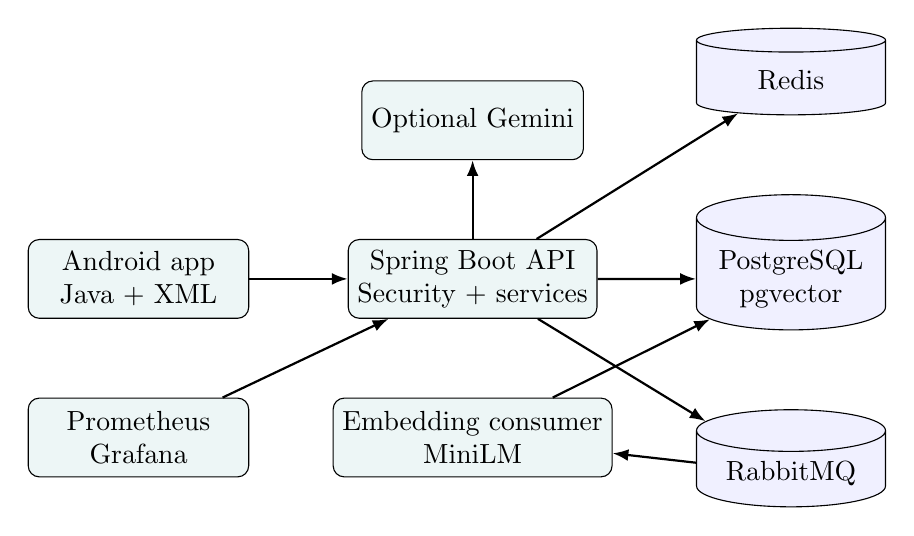
\begin{tikzpicture}[
node distance=1cm and 1.25cm,
box/.style={draw,rounded corners,align=center,minimum width=2.8cm,minimum height=1cm,fill=teal!7},
store/.style={draw,cylinder,shape border rotate=90,aspect=.28,align=center,minimum width=2.4cm,minimum height=1.1cm,fill=blue!6},
arr/.style={-{Latex[length=2mm]},thick}]
\node[box] (android) {Android app\\Java + XML};
\node[box,right=of android] (api) {Spring Boot API\\Security + services};
\node[store,right=of api] (pg) {PostgreSQL\\pgvector};
\node[store,above=of pg] (redis) {Redis};
\node[store,below=of pg] (rabbit) {RabbitMQ};
\node[box,below=of api] (worker) {Embedding consumer\\MiniLM};
\node[box,above=of api] (gemini) {Optional Gemini};
\node[box,below=of android] (obs) {Prometheus\\Grafana};
\draw[arr] (android)--(api);
\draw[arr] (api)--(pg);\draw[arr] (api)--(redis);\draw[arr] (api)--(rabbit);
\draw[arr] (rabbit)--(worker);\draw[arr] (worker)--(pg);
\draw[arr] (api)--(gemini);\draw[arr] (obs)--(api);
\end{tikzpicture}
\caption{EduFlex runtime architecture}\label{fig:architecture}
\end{figure}

\section{Backend structure}
Controllers define transport contracts and delegate to services. DTOs isolate wire
payloads from database records. Use-case classes perform validation and coordinate
repositories. Repositories contain JPA and jOOQ operations. Configuration supplies
security, caches, messaging, clocks, and metrics. This structure keeps business
invariants out of the mobile client and HTTP layer.

Figure~\ref{fig:backend-layers} makes the dependency direction explicit. Controllers
call application services, and services use repositories or integration clients.
Persistence code does not select HTTP responses, while Android does not calculate
authoritative rewards. These boundaries allow direct service testing and reduce the
effect of transport or database implementation changes.

\backendlayersdiagram

\section{Android structure}
Authentication activities lead to learner or administrator navigation. Learner
destinations include Home, Courses, Search, Cart, Profile, Payment, Course Detail,
Lesson Study, two quiz modes, Leaderboard, Reviews, Certificate, and AI Summary.
Administrator destinations include Users, Courses, Lessons, and Profile. API
interfaces, models, session managers, and list adapters support these screens.

Figure~\ref{fig:android-navigation} shows the learner path and the separate
administrator branch. Course Detail is a central decision screen that connects
discovery to enrolment, study, reviews, and AI support. Stable navigation IDs and
explicit arguments keep the course and lesson identity consistent across screens.

\androidnavigationdiagram

\section{Deployment}
The base Compose stack runs the API, PostgreSQL/pgvector, Redis, and RabbitMQ.
Named volumes preserve database and cache state through ordinary restarts. Health
checks order startup by dependency readiness. The monitoring overlay adds Prometheus,
Grafana, Alertmanager, Blackbox Exporter, PostgreSQL Exporter, and Redis Exporter.

Only selected interfaces are published to the host. PostgreSQL, Redis, exporters,
and the Actuator management listener remain on the Compose network. This reduces
accidental exposure while retaining local access to the API, RabbitMQ management,
and loopback monitoring tools. Figure~\ref{fig:deployment} shows the topology.

\deploymentdiagram

\section{Request and failure boundaries}
A mobile operation crosses the device-to-API boundary, the security-to-application
boundary, and usually an application-to-dependency boundary. Each can fail in a
different way. Connectivity failures produce a retryable mobile state. Authentication
and authorization failures return 401 or 403. Invalid input returns a validation
response. Transaction failures roll back related writes before an error leaves the
server.

This classification prevents an empty result from being confused with an error. An
empty catalogue is a successful query with no matching courses. A timeout, rejected
token, or unavailable database needs a distinct user message and operational signal.

\chapter{Database Design}
\section{Core model}
\begin{longtable}{p{0.25\textwidth}p{0.64\textwidth}}
\caption{Principal entity groups}\label{tab:entities}\\\toprule
\textbf{Group} & \textbf{Stored information}\\\midrule\endfirsthead
\toprule\textbf{Group} & \textbf{Stored information}\\\midrule\endhead
Users & Identity, BCrypt hash, profile, avatar, and role.\\
Courses and lessons & Metadata, price, images, lesson hierarchy, content, and media URL.\\
Quiz content & Questions, answer options, correct answers, and attempts.\\
Learning state & Enrolments, lesson completion, percentage, and timestamps.\\
Commerce and reviews & Payment records, ratings, text, and user-course relationships.\\
Gamification & XP, level, streaks, badges, badge awards, quests, and quest progress.\\
Semantic search & Course and lesson embeddings stored as pgvector columns.\\
\bottomrule
\end{longtable}

Figure~\ref{fig:erd} focuses on business relationships rather than listing every
column. Users and courses meet through enrolments, transactions, and reviews. Courses
contain lessons; lessons connect to progress, questions, and attempts. Gamification
is linked to the learner while badge definitions remain reusable across learners.

\erdmodeldiagram

\section{Ownership and lifecycle}
The user row is the root for authentication and learner-specific records. Removing a
user cascades through progress and quiz activity where migrations explicitly define
that behavior. A course owns its lesson hierarchy, and a lesson may reference a
parent lesson for grouped content. Questions belong to lessons and options belong to
questions. This ordering lets content deletion remove dependent assessment data in a
predictable direction.

Enrolment is the bridge between catalogue data and learner activity. The backend
checks it before accepting learning mutations. Progress records answer whether a
specific lesson transition happened; the enrolment holds the broader course state.
Gamification statistics aggregate learner rewards, while attempts retain assessment
history. Keeping these concepts separate allows an attempt to be audited without
recalculating an already awarded first-pass reward.

\section{Schema evolution}
The 27 migrations begin with users and progressively add courses, lessons, quizzes,
enrolments, gamification, payment, reviews, media, lesson hierarchy, embeddings,
quests, indexes, and constraint alignment. A clean database and an upgraded database
therefore reach the same versioned schema. Hibernate uses schema validation so drift
fails at startup. jOOQ source generation is explicit, allowing ordinary builds to
run without a developer database.

\section{Integrity and connections}
Foreign keys connect activity to users and content. Unique constraints protect
singular relationships such as enrolments and badge awards. Indexes support common
course, progress, ranking, and lookup paths. Constraints remain necessary even when
application code checks for an existing row because simultaneous transactions can
both pass a pre-insert check.

\begin{longtable}{p{0.27\textwidth}p{0.31\textwidth}p{0.31\textwidth}}
\caption{Selected integrity rules and their purpose}\label{tab:constraints}\\\toprule
\textbf{Data} & \textbf{Database rule} & \textbf{Invariant protected}\\\midrule\endfirsthead
\toprule\textbf{Data} & \textbf{Database rule} & \textbf{Invariant protected}\\\midrule\endhead
Enrolment & Unique user--course pair & A learner joins a course once.\\
Lesson progress & Unique user--lesson pair & One authoritative completion transition exists.\\
Gamification statistics & Unique user identifier & Concurrent initialization cannot create two totals.\\
Badge award & Unique user--badge pair & A badge definition may be reused but its award is singular per learner.\\
Course review & Unique user--course pair & A learner maintains one review for a course.\\
Daily quest progress & Unique user--quest--date tuple & Daily work cannot create duplicate counters.\\
Badge definition & Unique condition type & Concurrent course completion reuses one definition.\\
Dependent learning rows & Foreign keys with selected cascades & User and content deletion has a defined direction.\\
\bottomrule
\end{longtable}

HikariCP defaults to a maximum pool of 10 and two idle connections. Open Session in
View is disabled, preventing lazy database work during response rendering. Pool
active, maximum, and pending counts are exported as metrics.

\section{Relational and vector data together}
Embedding columns live beside course and lesson records, so semantic retrieval can
apply normal relational filters before similarity ordering. A course question first
restricts candidate material to the requested course and only then ranks vector
distance. The benefit is one transaction and backup boundary for content and vectors.
The trade-off is that embedding dimensions and extension availability become part of
the PostgreSQL schema and migration process.

The current MiniLM model produces 384 values. A future model change with a different
dimension would require a planned migration and complete re-embedding. Recording the
model identity with future vectors would make mixed-model transitions safer.

\chapter{Mobile Application Implementation}
\section{User experience}
The UI shares a Material 3 theme, colors, typography, cards, and bottom navigation.
Home presents learner status and continuation. Discover and Search expose the
catalogue. My Learning shows enrolments. Course Detail links to study, reviews, and
AI assistance. Profile and gamification screens present personal progress.

Data-driven screens explicitly show loading, empty results, and retryable failures.
This prevents a blank screen from being interpreted as success or a crash.

The learner journey in Figure~\ref{fig:learner-journey} connects UI decisions to
backend state changes. Free and paid courses converge on one enrolment concept.
Content and quiz lessons also converge before reward evaluation, which keeps the
mobile interface focused on interaction while the backend determines correctness.

\learnerjourneydiagram

After reward evaluation, an incomplete course returns the learner to the next available
lesson; completed courses retain their terminal completion state.

\begin{table}[H]\centering
\caption{Implemented learner screens and required visible states}\label{tab:ui-states}
\begin{tabular}{p{0.24\textwidth}p{0.31\textwidth}p{0.34\textwidth}}\toprule
\textbf{Screen} & \textbf{Successful content} & \textbf{Non-success state}\\\midrule
Home & Statistics and continuation cards & Loading, absent progress, retryable request failure\\
Discover/Search & Course cards and filtered results & Loading, empty result, clear query, retry\\
My Learning & Enrolled course list & Empty route back to discovery, retry\\
Course Detail & Metadata, enrol/study, reviews, AI entry & Loading, missing course, network failure\\
Lesson/Quiz & Content, question, answer feedback & Validation, submission failure, preserved context\\
Profile/Rewards & Profile, XP, quests, badges & Loading, empty rewards, retry\\
\bottomrule\end{tabular}
\end{table}

The table is a source-level inventory, not a usability result. The recorded emulator
journey observed authentication, Home, Learn, and successful authenticated calls, but
it did not capture submission-quality screenshots or cover every state. A final report
submission should include annotated device captures only after repeating the journey
with non-sensitive demonstration data.

\section{Networking and authentication}
The API URL is injected into \texttt{BuildConfig}; the emulator default is
\url{http://10.0.2.2:8080/}. Retrofit interfaces map each backend domain.
Debug builds enable HTTP logging and release builds disable it. After login, session
management stores the access token, refresh token, role, and profile information.
Provider secrets are never placed in Android build configuration.

The token manager gives networking code one location for bearer credentials. API
interfaces are divided by domain so course browsing does not depend on administrator
or payment details. Request and response models mirror the wire contract. This design
is intentionally pragmatic for the project scale: fragments coordinate their screen
state and adapters render collections, while authoritative rules remain on the server.

When a request fails, the screen retains enough context to retry without losing the
selected course. Authentication failures lead back to a valid session path; ordinary
network failures keep a retry action close to the failed content. Debug HTTP logging
supports development diagnosis, and disabling it in release avoids routine token and
payload exposure in release logs.

\section{Learning and engagement}
Lessons render content or open multiple-choice and fill-in-the-blank quiz flows.
Quiz results are sent to the backend so correctness, first-pass rewards, quests, and
completion are decided centrally. Gamification displays XP, levels, streaks, quests,
badges, and leaderboard position. WorkManager provides local reminders; optional
Firebase Messaging provides remote notifications.

Course completion is derived from required content and assessment state rather than
from a button controlled by the device. The client submits the event and renders the
returned result. This allows another device or a retried request to observe the same
server state. The progress state model is discussed in the reliability chapter.

\section{UI quality and accessibility considerations}
Material components provide consistent touch targets, typography, colors, and control
behavior. Lists use dedicated empty views rather than leaving an empty RecyclerView.
Search supports keyboard submission, clearing, and retry. My Learning offers a route
back to discovery when the learner has no enrolments.

The acceptance checklist includes normal and enlarged fonts, keyboard visibility,
back navigation, loading, empty, and offline states. Further accessibility work should
add automated contrast and content-description checks plus TalkBack traversal tests.
Those checks are proposed work and are not claimed as completed evaluation.

\section{Build variants}
The debug APK is installable for development. The release variant enables minification,
optimization, and resource shrinking. CI verifies release APK and AAB generation,
but the artifacts remain unsigned and are not store-ready.

\chapter{Backend and Security Implementation}
\section{REST API}
Routes cover users, authentication, courses, lessons, enrolment, progress, quizzes,
payments, reviews, media, gamification, badges, quests, and administration.
Swagger UI is available at \texttt{/swagger-ui/index.html} and OpenAPI at
\texttt{/v3/api-docs}. Validation and centralized exception handling make input and
failure responses consistent.

The API is organized around resources rather than individual screens. Android may
change its navigation without renaming the progress or course contract. Read routes
return DTOs shaped for clients; commands accept JSON, form data, or multipart content
according to the operation. Figure~\ref{fig:api-boundaries} groups routes by the
security decision that protects them.

\apiboundarydiagram

\section{API contract groups}
Account contracts create sessions and maintain profiles. Catalogue contracts return
courses, search results, owned courses, reviews, summaries, and grounded answers.
Learning contracts cover enrolment, lesson hierarchy, progress, and the two quiz
submission forms. Gamification contracts return statistics, check-in results, quests,
badges, and leaderboard entries. Media uses multipart requests because binary content
has different validation and size requirements from JSON.

Administrative commands are collected under \texttt{/api/admin} for list, create,
update, and delete workflows, with additional privileged mutations explicitly covered
by security rules. The complete generated contract remains available through OpenAPI;
the report groups related endpoints so the reader can understand responsibility and
access without reproducing a large machine-generated document.

\begin{longtable}{p{0.19\textwidth}p{0.70\textwidth}}
\caption{Representative API contracts}\label{tab:api-contracts}\\\toprule
\textbf{Operation} & \textbf{Contract, success, and failure boundary}\\\midrule\endfirsthead
\toprule\textbf{Operation} & \textbf{Contract, success, and failure boundary}\\\midrule\endhead
Login & POST \url{/api/user/login} accepts email and password. Success returns access and refresh tokens, user, and role; validation or invalid credentials fail.\\
Refresh & POST \url{/api/auth/refresh} accepts a refresh token. Success returns a new access token; an unknown user or malformed token returns 400, and an expired or revoked token returns 401.\\
Enrol & POST \url{/api/enrollment/{courseId}/register} accepts the user ID. Success creates the singular learner-course enrolment; unauthenticated and wrong-owner calls are rejected.\\
Complete lesson & POST \url{/api/progress/lesson} accepts form fields \texttt{lessonId} and \texttt{userId}. Success returns the progress percentage after a protected transition; invalid ownership, enrolment, or lesson state fails.\\
Submit quiz & POST \url{/api/quiz/submit-multiple-choice} accepts user, lesson, and answers. Success returns score, course progress, XP, and completed quests; a response-loss retry may add an attempt.\\
Ask course & POST \url{/api/course/{courseId}/ask} accepts a question of at most 500 characters. Success returns an answer, lesson sources, and provider flag; provider failure uses the fallback.\\
\bottomrule
\end{longtable}

The progress command remains form-encoded for compatibility with the Android client.
A representative successful response is:
\begin{lstlisting}[language={},caption={Lesson-completion response contract}]
{
  "success": true,
  "message": "Lesson progress saved",
  "newProgressPercent": 50.0
}
\end{lstlisting}
The request has no client idempotency key. Protected idempotency comes from the unique
user--lesson row and conditional transaction. Quiz attempts have a different boundary
and can still duplicate history after a lost response, as discussed later.

\section{Authentication and authorization}
Passwords use BCrypt. Login returns a 15-minute access token with identity, email,
role, and token type, plus a 30-day refresh token with a unique identifier. Refresh
state is held in Redis and logout revokes it. Spring Security uses stateless sessions.
Public routes include registration, login, recovery, refresh, logout, health, and
API documentation. Other routes require authentication. Administrator operations
require the \texttt{ADMIN} role; learning mutations also validate ownership.

Figure~\ref{fig:auth-sequence} follows both the initial login and later refresh.
The access token is self-contained and short-lived. The refresh token is longer-lived,
but its identifier is checked in Redis, which gives logout a server-side revocation
point. A refresh token is not accepted as an access token because the signed token
also carries a token-type claim.

Logout deletes the selected refresh-token record. It prevents that refresh token from
minting another access token; it does not immediately invalidate an already issued
15-minute access token. This bounded residual session is a consequence of stateless
access-token validation.

\authsequencediagram

Authorization has two levels. Route rules decide whether a role may reach an endpoint.
Application rules then check whether the authenticated learner owns the requested
user path and is enrolled in the relevant course. Role checks alone cannot protect a
request such as ``save progress for user B'' made by authenticated user A.

\section{Media}
The server can upload avatars, course images, and lesson videos to Supabase Storage
when configured. The secret stays on the backend. The core service can run without
these optional credentials.

\section{Redis cache policy}
\begin{table}[H]\centering
\caption{Configured Redis cache lifetimes}\label{tab:cache}
\begin{tabular}{lr@{\qquad}lr}\toprule
Courses & 5 min & Lessons & 5 min\\
Quizzes & 10 min & Leaderboard & 1 min\\
User statistics & 2 min & Badge catalogue & 30 min\\
User badges & 5 min & Reviews & 3 min\\
Course catalogue & 5 min & AI summaries & 6 hours\\
Semantic search & 15 min & &\\\bottomrule
\end{tabular}
\end{table}
Writes evict relevant entries. Embedding processing clears semantic and summary
results affected by changed content. Cache statistics support measurement.

Figure~\ref{fig:cache-flow} shows the cache-aside behavior. A cache hit avoids a
database query. A miss loads authoritative data and stores a bounded copy. Mutations
evict domain caches rather than attempting to modify several serialized cached
representations in place.

\cacheflowdiagram

Short TTLs are used for rapidly changing learner state, while the badge catalogue
and generated summaries can live longer. This is a consistency trade-off, not a
guarantee that data remains unchanged for the whole TTL. Explicit eviction narrows
the stale interval after known writes; expiration protects against missed eviction
and limits memory growth.

\chapter{Reliability, Concurrency, and Messaging}
\section{Transactional updates}
One learning action may update progress, XP, quests, enrolment completion, and
badges. These operations run inside one transaction. If an injected failure occurs
after intermediate writes, all changes roll back and a later retry completes once.

\section{Per-learner serialization}
The service locks the learner's statistics row with PostgreSQL
\texttt{SELECT FOR UPDATE}. Requests for one learner serialize at the critical
transition, while different learners proceed independently. Conditional updates
decide whether a transition is new and uniqueness constraints provide a final
safeguard. Protected transitions include lesson completion, daily check-in,
enrolment, first quiz pass, course completion, quest completion, and badge award.

Figure~\ref{fig:progress-state} shows the lifecycle seen by repeated requests. A
duplicate does not reverse the learner or create a second protected reward; it returns
the state that already won the race. This property matters on mobile networks, where
the server may commit even when the client never receives the response.

\progressstatediagram

\begin{figure}[H]\centering
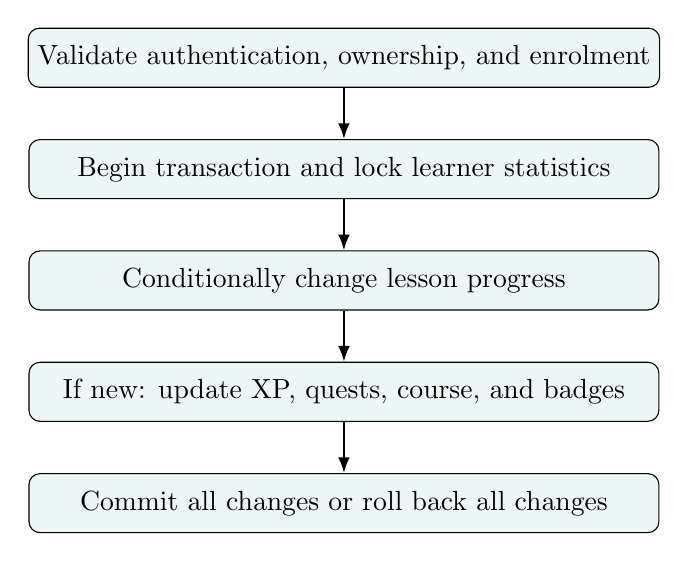
\begin{tikzpicture}[node distance=.65cm,
processbox/.style={draw,rounded corners,fill=teal!7,align=center,minimum width=8cm,minimum height=.75cm},
arr/.style={-{Latex[length=2mm]},thick}]
\node[processbox](a){Validate authentication, ownership, and enrolment};
\node[processbox,below=of a](b){Begin transaction and lock learner statistics};
\node[processbox,below=of b](c){Conditionally change lesson progress};
\node[processbox,below=of c](d){If new: update XP, quests, course, and badges};
\node[processbox,below=of d](e){Commit all changes or roll back all changes};
\draw[arr](a)--(b);\draw[arr](b)--(c);\draw[arr](c)--(d);\draw[arr](d)--(e);
\end{tikzpicture}
\caption{Concurrency-safe progress transaction}\label{fig:progress}
\end{figure}

\section{RabbitMQ embeddings}
Course and lesson services publish a content-change event after transaction commit.
A durable queue feeds a listener with prefetch 10 and three retry attempts. The
listener creates a MiniLM vector, stores it, and invalidates related caches.
Publication outcomes and processing duration are measured.

Figure~\ref{fig:embedding-sequence} explains the ordering. Publishing before commit
could let the consumer read old content or embed a write that later rolls back.
After-commit publication avoids that ordering error and keeps model inference outside
the HTTP response time.

\embeddingsequencediagram

The design currently has no transactional outbox or publisher confirmation. A
committed content write can therefore exist without a durable event if publication
fails. Operators must react to the alert and replay affected content.

\section{Known retry boundary}
Quiz submissions create attempt records and do not accept a client idempotency key.
A response-loss retry can create another attempt and increment an unfinished quest.
First-pass XP, course XP, quest-completion XP, progress, and badges remain protected.

\section{Failure analysis}
\begin{longtable}{p{0.27\textwidth}p{0.32\textwidth}p{0.30\textwidth}}
\caption{Reliability mechanisms and remaining boundaries}\\\toprule
\textbf{Failure} & \textbf{Current protection} & \textbf{Remaining action}\\\midrule\endfirsthead
\toprule\textbf{Failure} & \textbf{Current protection} & \textbf{Remaining action}\\\midrule\endhead
Duplicate lesson request & Conditional transition and unique model & Return existing state without new XP.\\
Concurrent reward writes & Per-learner row lock and transaction & Observe lock time and pool pressure.\\
Exception after partial work & Transaction rollback & Retry the complete operation.\\
RabbitMQ publish failure & Content stays committed; failure metric increases & Replay content and add an outbox.\\
Consumer failure & Listener retries three times & Add explicit dead-letter handling.\\
Lost quiz response & Protected rewards remain single & Add an idempotency key for attempts.\\
Redis unavailable & Readiness and monitoring expose dependency failure & Restore Redis and define degraded behavior.\\
\bottomrule
\end{longtable}

Correctness and throughput have different meanings. Serializing one learner's reward
mutations is intentional because those operations contend for one logical aggregate.
Different learners lock different rows and can proceed independently. A load test is
still required to measure connection-pool, database CPU, and lock-duration limits.

\chapter{AI-Assisted Learning}
\section{Retrieval}
The local all-MiniLM-L6-v2 model produces 384-dimensional course and lesson vectors.
A learner question is embedded and compared with chunks from the selected course
using pgvector. Constraining retrieval by course reduces unrelated context.

Embedding is a representation step rather than an answer-generation step. Vector
distance lets differently worded questions locate related lessons. The relational
course filter still defines the permitted knowledge boundary: SQL supplies ownership
and scope, while vector similarity supplies relevance.

\section{Grounded generation and fallback}
Retrieved chunks become context for optional Gemini generation. The result contains
source information so the UI can identify supporting material. Expensive summaries
and search results are cached. Without \texttt{GEMINI\_API\_KEY}, summaries use a
deterministic overview and questions return retrieved lesson suggestions, allowing
local development and tests without provider access.

The backend returns sources with the answer instead of presenting generated prose
alone. This gives the learner a route back to the lesson and lets an evaluator inspect
retrieval quality. If retrieval selects weak evidence, fluent wording does not make
the evidence stronger; source visibility makes the weakness observable.

\begin{figure}[H]\centering
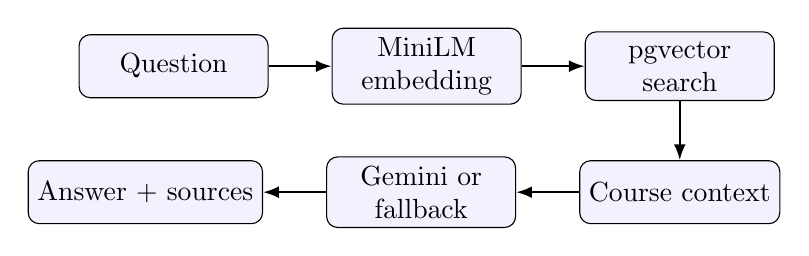
\begin{tikzpicture}[node distance=.75cm and .8cm,
box/.style={draw,rounded corners,align=center,fill=blue!5,minimum width=2.4cm,minimum height=.8cm},
arr/.style={-{Latex[length=2mm]},thick}]
\node[box](q){Question};\node[box,right=of q](e){MiniLM\\embedding};
\node[box,right=of e](s){pgvector\\search};
\node[box,below=of s](c){Course context};
\node[box,left=of c](g){Gemini or\\fallback};
\node[box,left=of g](a){Answer + sources};
\draw[arr](q)--(e);\draw[arr](e)--(s);\draw[arr](s)--(c);
\draw[arr](c)--(g);\draw[arr](g)--(a);
\end{tikzpicture}
\caption{Grounded course-question flow}\label{fig:rag}
\end{figure}

\section{Responsible boundaries}
Prompts, learner IDs, emails, tokens, and questions are excluded from metric labels.
Answers remain attributable to stored course content and are not treated as
authoritative academic assessment. Provider outcomes use bounded metric labels.

\section{Quality evaluation approach}
The current automated test proves deterministic fallback behavior. A broader AI
evaluation should prepare representative questions for each course, expected lesson
sources, and educator-reviewed answer criteria. Retrieval can then be measured through
source recall and ranking, while generated responses can be judged for groundedness,
completeness, and unsupported claims. Latency and provider failure rate should be
reported separately from content quality.

This evaluation remains future work because the repository does not contain a labelled
educational benchmark. The report describes the implemented retrieval pipeline without
claiming a measured pedagogical quality threshold.

\chapter{DevOps, Deployment, and Monitoring}
\section{Containerization and configuration}
Docker Compose builds the API and runs PostgreSQL/pgvector, Redis with append-only
persistence, and RabbitMQ. Health checks guard dependency readiness. Example
environment files document variable names; real credentials stay untracked.

\section{Continuous integration}
GitHub Actions runs three dependent jobs. The backend job uses JDK 21 and executes
Maven/Testcontainers tests. The monitoring job starts an isolated stack and validates
it. The Android job installs SDK 35, runs lint, builds debug and release APKs, and
builds a release AAB. Reports and artifacts are retained for 14 days.

\begin{figure}[H]\centering
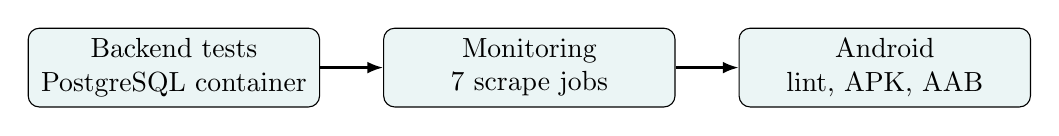
\begin{tikzpicture}[node distance=.8cm,
job/.style={draw,rounded corners,fill=teal!8,align=center,minimum width=3.7cm,minimum height=1cm},
arr/.style={-{Latex[length=2mm]},thick}]
\node[job](b){Backend tests\\PostgreSQL container};
\node[job,right=of b](m){Monitoring\\7 scrape jobs};
\node[job,right=of m](a){Android\\lint, APK, AAB};
\draw[arr](b)--(m);\draw[arr](m)--(a);
\end{tikzpicture}
\caption{Continuous integration order}\label{fig:ci}
\end{figure}

\section{Metrics, dashboards, and alerts}
Actuator and Micrometer expose JVM, HTTP, HikariCP, and custom metrics on an internal
management listener. Prometheus scrapes the API, its main-listener probe, PostgreSQL,
Redis, and RabbitMQ exporters \cite{prometheus}. Custom metrics cover progress, rewards, statistics-lock
duration, embedding publication and processing, and AI outcomes.

Grafana provisions Service Overview, Dependencies, and Learning Operations dashboards
\cite{grafana}.
Alerts cover API availability, absent targets, 5xx rate, p95 latency, pool contention,
queue backlog, absent consumers, publication failure, RabbitMQ alarms, Redis evictions,
and PostgreSQL deadlocks. Alertmanager groups alerts locally.

Figure~\ref{fig:monitoring-flow} separates telemetry sources from storage, display,
and local alert inspection. A healthy Actuator scrape proves that the management listener is
alive; the Blackbox probe separately tests the client-facing API port. The two signals
prevent a healthy metrics port from hiding a failed application listener.

\monitoringflowdiagram

\begin{figure}[H]\centering
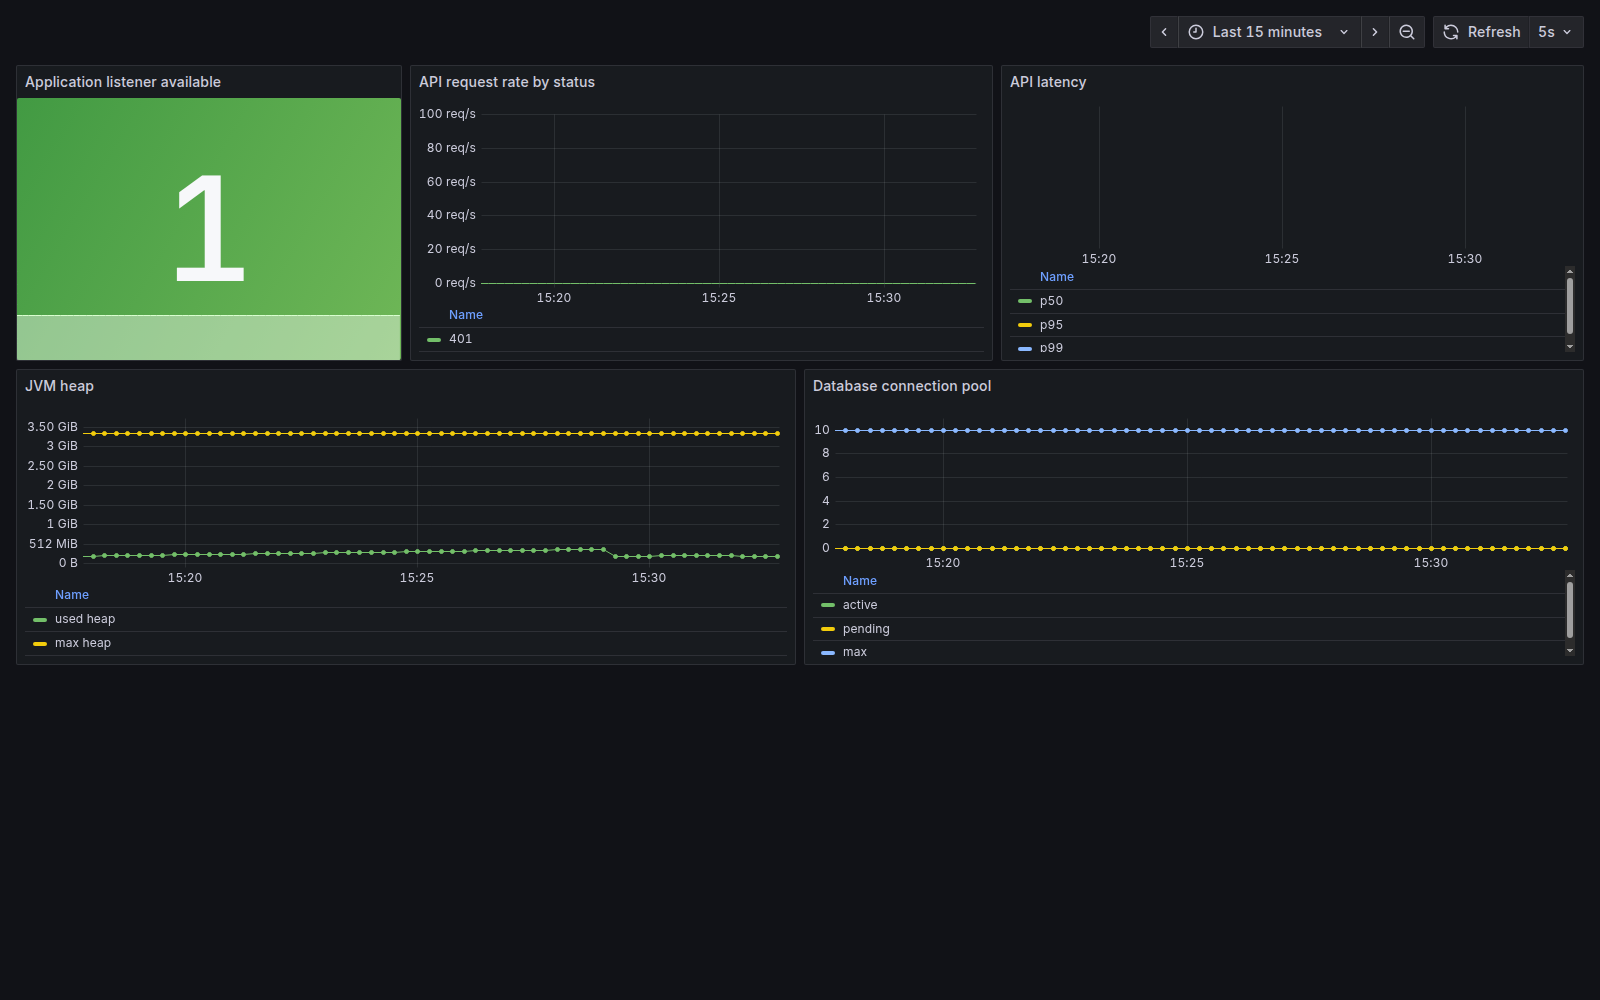
\includegraphics[width=\textwidth]{figures/grafana-service-overview.png}
\caption{Provisioned Grafana Service Overview running against the local stack}
\label{fig:grafana-overview}
\end{figure}

Figure~\ref{fig:grafana-overview} is a real local capture rather than a mock-up. It
shows the independent application-listener probe, request status, latency panels, JVM
heap, and Hikari connection-pool capacity. The near-idle request and latency panels
reflect the capture workload; they must not be interpreted as a benchmark.

\section{Operational security}
Liveness and readiness are exposed on the main API port. The monitoring profile
exposes only health and Prometheus on internal port 8081. Grafana, Prometheus, and
Alertmanager bind to loopback locally. The PostgreSQL exporter uses a dedicated
\texttt{eduflex\_monitor} role with \texttt{pg\_monitor}. Prometheus retention is
bounded to seven days or 2 GB.

The current Alertmanager receiver groups alerts for inspection in its local web UI but
does not send email, chat, or paging notifications. External delivery is therefore a
future deployment task rather than an implemented operational guarantee.

\section{Operational interpretation}
The dashboards correspond to questions asked during an incident. Service Overview
shows whether the API is unreachable, slow, failing, or waiting for database
connections. Dependencies narrows pressure to PostgreSQL, Redis, or RabbitMQ.
Learning Operations shows progress transitions, rewards, row-lock time, embedding
work, and AI outcomes.

An alert starts an investigation; it does not prove one cause. High latency together
with Hikari pending requests points toward database work or pool saturation. A growing
embedding queue with zero consumers points toward listener startup or broker
connectivity. Redis eviction requires inspecting memory policy and workload before
capacity changes. The monitoring runbook records these decision paths and recovery
checks.

\chapter{Testing and Evaluation}
\section{Strategy}
Verification combines unit tests, database integration tests, live API journeys,
Android emulator checks, lint, builds, and monitoring smoke tests. Attention focuses
on token semantics, rollback, ownership, duplicate rewards, concurrency, and startup.

Unless a row states otherwise, the recorded evidence was produced on 24--25 September
2026 from Git revision \texttt{3d21d21} on branch
\path{dev/set-up-message-queue}. The detailed scenario record is versioned in
\path{docs/reliable-progress-verification.md}; monitoring procedures and the dated
smoke result are in \texttt{docs/monitoring-runbook.md}. Naming the revision matters:
test totals are historical observations and must be rerun after functional changes.

No single test layer proves the whole system. Unit tests give fast feedback for token
and fallback behavior. Testcontainers supplies real transaction, constraint, and lock
semantics. The live API journey checks security filters, serialization, persistence,
and messaging through HTTP. The emulator adds Android navigation and contract mapping.
Monitoring verification confirms that operational signals remain usable after startup.

\begin{table}[H]\centering
\caption{Evidence mapped to quality goals}\label{tab:evidence}
\begin{tabular}{p{0.25\textwidth}p{0.32\textwidth}p{0.32\textwidth}}\toprule
\textbf{Goal} & \textbf{Evidence} & \textbf{What it establishes}\\\midrule
Security & JWT tests and rejected HTTP flows & Token type, role, and ownership in tested routes.\\
Consistency & PostgreSQL concurrency suite & Single protected transitions under duplicate calls.\\
Atomicity & Injected transaction failure & Related progress and rewards roll back together.\\
Integration & 26-check live HTTP journey & Main backend workflow across real dependencies.\\
Mobile compatibility & Contract test and API 35 emulator & Token mapping and representative navigation.\\
Delivery & Lint, APK, and AAB builds & Source and shrinking configuration compile.\\
Observability & Targets, dashboards, and alert drill & Metrics and alert lifecycle work locally.\\
\bottomrule\end{tabular}
\end{table}

\begin{longtable}{p{0.27\textwidth}p{0.31\textwidth}p{0.31\textwidth}}
\caption{Claim-to-evidence traceability}\label{tab:traceability}\\\toprule
\textbf{Report claim} & \textbf{Repository evidence} & \textbf{Boundary}\\\midrule\endfirsthead
\toprule\textbf{Report claim} & \textbf{Repository evidence} & \textbf{Boundary}\\\midrule\endhead
Protected rewards are single under duplicate concurrency & Progress concurrency integration test; final database assertions after 100 synchronized calls & Correctness for defined scenarios, not capacity\\
Related writes are atomic & Injected exception and retry integration scenario & One transaction path and PostgreSQL configuration\\
Authorization rejects wrong ownership & Integration scenarios plus live HTTP journey & Exercised routes, not a complete penetration test\\
Embedding crosses RabbitMQ & HTTP journey waits for stored vector after content change & Successful delivery path; no outbox guarantee\\
Refresh revocation works & JWT unit tests and refresh/logout HTTP checks & Refresh token only; issued access token remains valid until expiry\\
Android consumes the contract & Login response unit test and API 35 emulator journey & Representative navigation, not full device coverage\\
Monitoring detects API loss & Versioned rules, seven targets, and stop/recovery drill & Local Compose; receiver has no external notification route\\
Release source compiles with shrinking & Gradle release APK/AAB tasks & Unsigned inspection artifacts\\
\bottomrule
\end{longtable}

\section{Backend results}
The recorded run used Java 21, Docker Engine 29.8.1, and PostgreSQL 16/pgvector.
All 27 migrations ran. The result was 20 tests with zero failures, errors, or skips;
18 scenarios belong to the progress concurrency integration suite.

\begin{longtable}{p{0.58\textwidth}p{0.30\textwidth}}
\caption{Selected verified scenarios}\label{tab:tests}\\\toprule
\textbf{Scenario} & \textbf{Observed result}\\\midrule\endfirsthead
\toprule\textbf{Scenario} & \textbf{Observed result}\\\midrule\endhead
100 concurrent completions of one lesson & One progress row and exactly 20 XP.\\
100 concurrent daily check-ins & One date transition and exactly 10 XP.\\
100 concurrent first statistics reads & One row without uniqueness failure.\\
Repeated lesson completion & Timestamp and XP preserved.\\
Different lessons completed concurrently & Both rewards and percentage correct.\\
Concurrent first quiz passes & First-pass and course XP awarded once.\\
Two learners complete one course & One badge definition and one award per learner.\\
Injected failure after related writes & Full rollback; retry succeeds once.\\
Unauthorized and wrong-owner calls & Rejected without state mutation.\\
Daily boundary with fixed clock & Same-day, next-day, zone, and future cases pass.\\
\bottomrule
\end{longtable}
These tests establish correctness for the tested cases; they are not a throughput
benchmark and do not claim production latency.

The concurrency harness starts 100 worker threads together and permits up to 32
simultaneous test database transactions. Assertions inspect final database state,
not only successful responses. This matters because every call could return success
while still duplicating XP internally. A pinned PostgreSQL/pgvector image and Flyway
startup keep tested database behavior close to the local runtime.

\section{End-to-end and Android results}
A live HTTP journey completed 26 checks with no failures. It covered administrator
and learner registration, protected content creation, catalogue reads, cross-user
rejection, enrolment, progress, quiz retry, XP totals, embedding completion, refresh,
logout, and revoked-token rejection.

The debug APK was exercised on an Android 15 API 35 emulator. A learner registered,
logged in, opened the main activity, accepted notification permission, viewed Home,
opened Learn, and received successful authenticated statistics, quest, and enrolment
responses. A unit contract test protects access-token response mapping.

The journey also waited for RabbitMQ embedding completion, demonstrating that a
content update can travel through broker and consumer into vector storage. It checked
token refresh followed by logout and rejection of the revoked token. These steps join
otherwise isolated features into a meaningful lifecycle.

\section{Build and monitoring results}
Android debug lint, debug APK, release APK, and release AAB tasks succeeded with
release shrinking enabled. Monitoring verification checked Compose configuration,
alert rules, metric protection, seven Prometheus jobs, and three dashboards.
A controlled API stop caused the availability alert to fire after one minute and
resolve after recovery.

The drill checks both directions of the alert lifecycle. Firing demonstrates detection;
resolution confirms that the rule, scrape path, and restored service agree after
recovery instead of leaving a stale incident.

\section{Evaluation limits}
Emulator checks do not cover every device, screen size, or accessibility setting.
No formal usability study or load-test dataset has been completed. External providers
require separate credentials. These limits prevent unsupported claims and define
future evaluation work.

A formal next evaluation should record task completion time and error rate for new
learners, accessibility findings, p50/p95/p99 latency under a defined workload,
database and queue saturation points, and recovery time after dependency failures.
Each result should state dataset size, hardware, concurrency, cache state, and the
script used to reproduce it.

\section{Performance claims and missing measurements}
Redis and RabbitMQ change where work occurs, but their presence alone does not prove a
performance improvement. The project has not yet recorded uncached versus cached
latency, synchronous versus queued embedding response time, sustained throughput, or
resource saturation. Consequently, this report describes the intended performance
mechanism and does not attach numerical speed-up claims to it.

\begin{table}[H]\centering
\caption{Required performance experiment design}\label{tab:performance-plan}
\begin{tabular}{p{0.26\textwidth}p{0.31\textwidth}p{0.32\textwidth}}\toprule
\textbf{Question} & \textbf{Controlled comparison} & \textbf{Reportable measures}\\\midrule
Does caching help? & Cold/miss, warm/hit, and post-eviction reads with the same dataset & p50/p95/p99 latency, database calls, hit ratio\\
Does queuing shorten writes? & Content update with synchronous embedding baseline versus post-commit publication & HTTP latency, queue delay, end-to-end embedding time\\
Where does concurrency saturate? & Increasing learners and requests with fixed hardware and pool settings & Throughput, errors, lock time, CPU, pool pending\\
How does failure recover? & Stop and restore Redis, RabbitMQ, API, and consumer independently & Detection time, recovery time, lost/replayed work\\
\bottomrule\end{tabular}
\end{table}

\chapter{Conclusion and Future Work}
\section{Conclusion}
EduFlex delivers a mobile learning experience supported by a secure, transactional,
and observable backend. It covers the path from Material-based Android screens to
REST services, relational storage, caches, messaging, semantic retrieval, integration
tests, containers, and dashboards.

The central achievement is trustworthy learning state. Progress and gamification are
coordinated through transactions, row locks, conditional transitions, and constraints.
Tests demonstrate that concurrent duplicate calls do not duplicate protected rewards.
Caching and asynchronous embedding improve the design without moving authority away
from PostgreSQL.

Observability is part of the implementation: metrics represent infrastructure and
learning operations, dashboards are version-controlled, and availability alerting
has been exercised. CI combines backend correctness, monitoring, and Android delivery.

\section{Future work}
\begin{enumerate}[leftmargin=*]
\item add a transactional outbox, publisher confirmation, and reconciliation;
\item add client idempotency keys and a reward ledger for quiz and payment retries;
\item add structured centralized logs and OpenTelemetry traces;
\item configure external alert delivery and encrypted backups with restore drills;
\item load-test catalogue, progress, and AI paths and define measured objectives;
\item expand Android instrumentation, accessibility, offline, and device testing;
\item implement secure release signing and an approved store workflow; and
\item evaluate AI answers with a labelled dataset and educator review.
\end{enumerate}

\section{Portfolio summary}
\begin{quote}
Designed and implemented a native Android learning platform with a Spring Boot API,
PostgreSQL/pgvector, Redis, RabbitMQ, JWT security, grounded AI assistance, and
Prometheus with Grafana. Built concurrency-safe progress and reward
transactions and verified single-reward behavior under 100 simultaneous duplicate
requests with Testcontainers.
\end{quote}

\appendix
\chapter{Build and Verification Commands}
\begin{lstlisting}[language=bash,caption={Start the base environment}]
cp .env.example .env
cp backend/.env.example backend/.env
docker compose --env-file backend/.env \
  -f backend/docker-compose.yml up --build -d
\end{lstlisting}
\begin{lstlisting}[language=bash,caption={Run backend tests}]
cd backend
./mvnw --batch-mode test
\end{lstlisting}
\begin{lstlisting}[language=bash,caption={Run Android verification}]
./gradlew --no-daemon \
  :app:lintDebug :app:assembleDebug \
  :app:assembleRelease :app:bundleRelease
\end{lstlisting}
\begin{lstlisting}[language=bash,caption={Verify monitoring}]
docker compose --env-file backend/.env \
  -f backend/docker-compose.yml \
  -f backend/docker-compose.monitoring.yml up --build -d
bash backend/scripts/verify-monitoring.sh
\end{lstlisting}

\chapter{Selected API Groups}
\begin{longtable}{p{0.28\textwidth}p{0.61\textwidth}}\toprule
\textbf{Route group} & \textbf{Responsibility}\\\midrule\endfirsthead
\toprule\textbf{Route group} & \textbf{Responsibility}\\\midrule\endhead
\texttt{/api/user} & Registration, login, recovery, and profile update.\\
\texttt{/api/auth} & Token refresh and logout.\\
\texttt{/api/course} & Catalogue, search, reviews, summary, and questions.\\
\texttt{/api/lesson} & Lesson creation and retrieval.\\
\texttt{/api/enrollment} & Learner enrolment and reads.\\
\texttt{/api/progress} & Lesson completion and course progress.\\
\texttt{/api/quiz} & Question retrieval and submissions.\\
\texttt{/api/payment} & Payment record processing.\\
\texttt{/api/users/...} & Statistics, streaks, quests, badges, and leaderboard.\\
\texttt{/api/media} & Avatar, image, and video upload.\\
\texttt{/api/admin} & Protected user and content administration.\\
\bottomrule\end{longtable}

\chapter{Configuration Reference}
\small
\begin{longtable}{p{0.38\textwidth}p{0.39\textwidth}p{0.10\textwidth}}
\toprule
\textbf{Variable} & \textbf{Purpose} & \textbf{Scope}\\\midrule\endfirsthead
\toprule\textbf{Variable} & \textbf{Purpose} & \textbf{Scope}\\\midrule\endhead
\texttt{API\_BASE\_URL} & Android REST endpoint, including trailing slash & Mobile\\
\texttt{SPRING\_DATASOURCE\_URL} & JDBC connection for direct backend execution & Backend\\
\texttt{SPRING\_DATASOURCE\_USERNAME} & Application database user & Backend\\
\texttt{SPRING\_DATASOURCE\_PASSWORD} & Application database password & Backend\\
\texttt{JWT\_SECRETKEY} & HMAC signing secret for access and refresh tokens & Backend\\
\texttt{REDIS\_PASSWORD} & Redis authentication & Infra\\
\texttt{RABBITMQ\_USERNAME} & Broker login name & Infra\\
\texttt{RABBITMQ\_PASSWORD} & Broker login password & Infra\\
\texttt{EDUFLEX\_TIME\_ZONE} & Calendar zone for streaks and daily rewards & Backend\\
\texttt{GEMINI\_API\_KEY} & Optional server-side generation credential & Optional\\
\texttt{GEMINI\_MODEL} & Optional generation model selection & Optional\\
\texttt{SUPABASE\_URL} & Optional media-storage project URL & Optional\\
\texttt{SUPABASE\_SECRET\_KEY} & Optional server-side storage credential & Optional\\
\texttt{GRAFANA\_ADMIN\_PASSWORD} & Local Grafana administrator password & Monitor\\
\texttt{POSTGRES\_MONITOR\_PASSWORD} & Dedicated exporter role password & Monitor\\
\texttt{EDUFLEX\_ENVIRONMENT} & Stable environment label on metrics & Monitor\\
\bottomrule
\end{longtable}
\normalsize

Real values belong in untracked environment files or a deployment secret store.
Provider keys and passwords must not appear in screenshots, source control, metric
labels, build logs, or the submitted report archive.

\chapter{Diagram and Evidence Index}
\begin{longtable}{p{0.31\textwidth}p{0.57\textwidth}}
\toprule
\textbf{View} & \textbf{Repository evidence represented}\\\midrule\endfirsthead
\toprule\textbf{View} & \textbf{Repository evidence represented}\\\midrule\endhead
System context & Android application, backend, optional Supabase, Gemini, and Firebase integrations.\\
Runtime architecture & Compose services, API dependency configuration, and embedding listener.\\
Backend layers & Controller, service, repository, security, configuration, and monitoring packages.\\
Android navigation & Learner and administrator navigation XML plus screen classes.\\
Deployment topology & Base and monitoring Compose files, exposed ports, and named volumes.\\
Database model & Flyway migrations, generated records, entities, and foreign keys.\\
API boundaries & Controller mappings and Spring Security route rules.\\
Authentication sequence & Login use case, JWT utility, refresh service, and Redis revocation.\\
Learner journey & Course, payment, enrolment, lesson, quiz, progress, and reward services.\\
Progress state & Conditional progress transitions and concurrency integration tests.\\
Cache flow & Redis configuration plus cacheable and eviction annotations.\\
Embedding sequence & After-commit publisher, RabbitMQ binding, listener, and embedding service.\\
AI retrieval & MiniLM embedding service, pgvector search, Gemini client, and fallback test.\\
CI flow & GitHub Actions backend, monitoring, and Android jobs.\\
Monitoring flow & Prometheus jobs and rules, exporters, Grafana provisioning, and Alertmanager.\\
\bottomrule
\end{longtable}

This index makes each visual auditable. The figures intentionally simplify class and
column detail, but their relationships follow the repository rather than a hypothetical
target architecture.

\chapter{Submission Checklist}
Replace title-page placeholders, use any declaration required by the institution,
and insert real screenshots. Confirm page-count and formatting rules, and update
verification dates after new test runs. Never include secrets, private Firebase
configuration, signing files, real user data, or access tokens in the report.

\bibliographystyle{plain}
\bibliography{references}
\end{document}
